%%%%%%%%%%%%%%%%%%%%%%%%%%%%%%%%%%%%%%%%%%%%%%%%%%%%%%%%%%%%%%%%%%%%
%%%%%%%%%%%%%%%%%%%%%%%%%%%%%%%%%%%%%%%%%%%%%%%%%%%%%%%%%%%%%%%%%%%%
%%                                                                %%
%% An example for writting your thesis using LaTeX                %%
%% Original version by Luis Costa,  changes by Perttu Puska       %%
%% Support for Swedish added 15092014                             %%
%%                                                                %%
%% This example consists of the files                             %%
%%         thesistemplate.tex (versio 2.01)                       %%
%%         opinnaytepohja.tex (versio 2.01) (for text in Finnish) %%
%%         aaltothesis.cls (versio 2.01)                          %%
%%         kuva1.eps                                              %%
%%         kuva2.eps                                              %%
%%         kuva1.pdf                                              %%
%%         kuva2.pdf                                              %%
%%                                                                %%
%%                                                                %%
%% Typeset either with                                            %%
%% latex:                                                         %%
%%             $ latex opinnaytepohja                             %%
%%             $ latex opinnaytepohja                             %%
%%                                                                %%
%%   Result is the file opinnayte.dvi, which                      %%
%%   is converted to ps format as follows:                        %%
%%                                                                %%
%%             $ dvips opinnaytepohja -o                          %%
%%                                                                %%
%%   and then to pdf as follows:                                  %%
%%                                                                %%
%%             $ ps2pdf opinnaytepohja.ps                         %%
%%                                                                %%
%% Or                                                             %%
%% pdflatex:                                                      %%
%%             $ pdflatex opinnaytepohja                          %%
%%             $ pdflatex opinnaytepohja                          %%
%%                                                                %%
%%   Result is the file opinnaytepohja.pdf                        %%
%%                                                                %%
%% Explanatory comments in this example begin with                %%
%% the characters %%, and changes that the user can make          %%
%% with the character %                                           %%
%%                                                                %%
%%%%%%%%%%%%%%%%%%%%%%%%%%%%%%%%%%%%%%%%%%%%%%%%%%%%%%%%%%%%%%%%%%%%
%%%%%%%%%%%%%%%%%%%%%%%%%%%%%%%%%%%%%%%%%%%%%%%%%%%%%%%%%%%%%%%%%%%%

%% Uncomment one of these:
%% the 1st when using pdflatex, which directly typesets your document in
%% pdf (use jpg or pdf figures), or
%% the 2nd when producing a ps file (use eps figures, don't use ps figures!).
\documentclass[english,12pt,a4paper,pdftex,sci,utf8]{aaltothesis}
%\documentclass[english,12pt,a4paper,dvips]{aaltothesis}

%% To the \documentclass above
%% specify your school: arts, biz, chem, elec, eng, sci
%% specify the character encoding scheme used by your editor: utf8, latin1

%% Use one of these if you write in Finnish (see the Finnish template):
%%
%\documentclass[finnish,12pt,a4paper,pdftex,elec,utf8]{aaltothesis}
%\documentclass[finnish,12pt,a4paper,dvips]{aaltothesis}

\usepackage{graphicx}
\usepackage[inkscapelatex=false]{svg}
\usepackage{tikz}
\usepackage[absolute,overlay]{textpos}
\usetikzlibrary{arrows.meta, positioning}
\usepackage{caption}
\usepackage{subcaption}
\usepackage{float} % For [H]
\usepackage[ruled]{algorithm2e}
\usepackage{threeparttable}
\usepackage{booktabs}
\SetKwComment{Comment}{/* }{ */}




%% Use this if you write hard core mathematics, these are usually needed
\usepackage{amsfonts,amssymb,amsbsy, amsmath}


%% Use the macros in this package to change how the hyperref package below 
%% typesets its hypertext -- hyperlink colour, font, etc. See the package
%% documentation. It also defines the \url macro, so use the package when 
%% not using the hyperref package.
%%
%\usepackage{url}

%% Use this if you want to get links and nice output. Works well with pdflatex.
\usepackage[hidelinks]{hyperref}
\hypersetup{pdfpagemode=UseNone, pdfstartview=FitH,
  colorlinks=true,urlcolor=red,linkcolor=blue,citecolor=black,
  pdftitle={Default Title, Modify},pdfauthor={Your Name},
  pdfkeywords={Modify keywords}}
\usepackage[capitalise,noabbrev]{cleveref}


\usepackage{float}


%% All that is printed on paper starts here
\begin{document}

%% Change the school field to specify your school if the automatically 
%% set name is wrong
 \university{aalto University}
 \school{School of Science}

%% Only for B.Sc. thesis: Choose your degree programme. 
\degreeprogram{Computer Science}
%%


%% Valitse yksi näistä kolmesta
%%
%% Choose one of these:
\univdegree{BSc}
%\univdegree{MSc}
%\univdegree{Lic}

%% Your own name (should be self explanatory...)
\author{Daniel Michaeli}

%% Your thesis title comes here and again before a possible abstract in
%% Finnish or Swedish . If the title is very long and latex does an
%% unsatisfactory job of breaking the lines, you will have to force a
%% linebreak with the \\ control character. 
%% Do not hyphenate titles.
%% 

\thesistitle{A Review of GPU Acceleration Techniques in Option Pricing Models}
\place{Espoo}

%% For B.Sc. thesis use the date when you present your thesis. 
%% 
%% Kandidaatintyön päivämäärä on sen esityspäivämäärä! 
\date{16.2.2025}

%% B.Sc. or M.Sc. thesis supervisor 
%% Note the "\" after the comma. This forces the following space to be 
%% a normal interword space, not the space that starts a new sentence. 
%% This is done because the fullstop isn't the end of the sentence that
%% should be followed by a slightly longer space but is to be followed
%% by a regular space.
%%
\supervisor{M.Sc.\ Henrik Lievonen} %{Prof.\ Pirjo Professori}

%% B.Sc. or M.Sc. thesis advisors(s). You can give upto two advisors in
%% this template. Check with your supervisor how many official advisors
%% you can have.
%%
%\advisor{Prof.\ Pirjo Professori}
%\advisor{D.Sc.\ (Tech.) Olli Ohjaaja}
\advisor{M.Sc.\ Henrik Lievonen}

%% Aalto logo: syntax:
%% \uselogo{aaltoRed|aaltoBlue|aaltoYellow|aaltoGray|aaltoGrayScale}{?|!|''}
%%
%% Logo language is set to be the same as the document language.
%% Logon kieli on sama kuin dokumentin kieli
%%
\uselogo{aaltoBlack}{''}

%% Create the coverpage
%%
\makecoverpage


%% Note that when writting your master's thesis in English, place
%% the English abstract first followed by the possible Finnish abstract

%% English abstract.
%% All the information required in the abstract (your name, thesis title, etc.)
%% is used as specified above.
%% Specify keywords
%%
%% Kaikki tiivistelmässä tarvittava tieto (nimesi, työnnimi, jne.) käytetään
%% niin kuin se on yllä määritelty.
%% Avainsanat
%%
\keywords{moi, mojn, moin, morjens, moro}
%% Abstract text
\begin{abstractpage}[english]

English bla bla bla
\end{abstractpage}

%% Force a new page so that the possible English abstract starts on a new page
%%
%% Pakotetaan uusi sivu varmuuden vuoksi, jotta 
%% mahdollinen suomenkielinen ja englanninkielinen tiivistelmä
%% eivät tule vahingossakaan samalle sivulle
\newpage
%

%% Force new page so that the Swedish abstract starts from a new page
\newpage
%
%% Swedish abstract. Delete if you don't need it. 
%% 
\thesistitle{Genomströmning och latens i datorsystem: en anlays av avvägningseffekter och optimeringsstrategier}
\advisor{M.Sc.\ Henrik Lievonen} %
\degreeprogram{Datateknik}
\department{Högskolan för teknikvetenskaper}%
\professorship{?}  %
%% Abstract keywords
\keywords{Nyckelord p\aa{} svenska,\\ Moi, moin, moidå, mojjdå}
%% Abstract text
\begin{abstractpage}[swedish]
 svenska bla bla bla
\end{abstractpage}

\newpage


%% Table of contents. 

\thesistableofcontents




%% Tweaks the page numbering to meet the requirement of the thesis format:
%% Begin the pagenumbering in Arabian numerals (and leave the first page
%% of the text body empty, see \thispagestyle{empty} below).
%% Additionally, force the actual text to begin on a new page with the 
%% \clearpage command.
%% \clearpage is similar to \newpage, but it also flushes the floats (figures
%% and tables).
%% There is no need to change these
%%
\cleardoublepage
\storeinipagenumber
\pagenumbering{arabic}
\setcounter{page}{1}


%% Text body begins. Note that since the text body
%% is mostly in Finnish the majority of comments are
%% also in Finnish after this point. There is no point in explaining
%% Finnish-language specific thesis conventions in English. Someday 
%% this text will possibly be translated to English.
%%
\section{Introduction}

%% Ensimm\"ainen sivu tyhj\"aksi
%% 
%% Leave first page empty
\thispagestyle{empty}
Options are financial contracts between two parties that grant the holder the right, but not the obligation, to buy or sell an underlying asset at a predetermined price by a future date \cite{hull2016options}. Options belong to a broader class of financial instruments known as derivatives, which derive their value from the price of the underlying asset. These instruments enable both speculative trading and risk management strategies, making them attractive even to non-financial institutions \cite{bartram2009international}. The derivatives market has experienced substantial growth over the past half-century, driven by advances in financial mathematics \cite{merton1994influence} and exponential increases in affordable computing power \cite{nordhaus2007two}.

Modern option pricing employs various models with different theoretical foundations and computational requirements. Execution speed is often critical. High-frequency trading strategies exploit transient market inefficiencies \footnote{A market inefficiency occurs when an asset price deviates from its theoretical fair value} through millions of rapid transactions, where millisecond delays can determine profitability. Faster computation also benefits risk management practices that rely on extensive portfolio simulations across multiple market scenarios. These performance requirements have motivated research into adapting option pricing algorithms to leverage the GPU's parallel computing capabilities.

This thesis presents a literature review 
of common option pricing algorithms' GPU acceleration potential and limitations. The aim is to assess how dependency structures in different algorithms affect their GPU parallelization potential, what approaches see the greatest performance improvements of a GPU implementation, analyze the scalability of these solutions, and identify related bottlenecks. I have chosen to analyze the Cox-Ross-Rubinstein (CRR) binomial option pricing model, and Monte Carlo (MC) simulation-based methods. The Black-Scholes analytical formula has been excluded as its GPU implementation is purely arithmetic evaluation with no algorithmic content. Methods requiring PDE numerical solutions would offer rich parallelization challenges but demand mathematical background beyond this thesis's scope.

The ~\cref{sec:theory} introduces formal definitions and fundamental option pricing theory. ~\cref{sec:gpu} presents a high-level overview of the GPU, how it differs architecturally from the CPU, and how it can be used for general-purpose computing. ~\cref{sec:gpu-crr},~\cref{sec:gpu-bsm}, and~\cref{sec:gpu-mc} review GPU implementations of each respective approach, considering the aforementioned factors. The results are summarized in ~\cref{sec:summary} and conclusions are drawn in ~\cref{sec:conclusions}.

For scope restriction purposes, the following choices have been made:
\begin{itemize}
\item Only European and American options are considered, with the exception of the Monte Carlo methods, which are particularly suitable for pricing exotic options with complex payoff structures. The term \emph{vanilla options} refers to both European and American options, whereas \emph{exotic options} denotes more complex contracts. Unless explicitly stated otherwise, all discussions and conclusions apply to options in general. When specific terms are used, the statements pertain strictly to those contract styles. Furthermore, it is assumed that the underlying asset does not pay a dividend.
    
\item The purpose of this paper is to draw general conclusions about the GPU acceleration potential for different option pricing approaches. The referenced research makes use of varying computing architectures and performance metrics. Other differences, like the number of active cores in the baseline CPU implementation, or the extent to which further optimizations have been implemented, also play a role. This makes direct quantitative comparisons difficult. To account for this limitation, the main comparisons of interest are the relative speedups of the GPU-accelerated implementations compared to their respective baseline solutions, and to a smaller extent relative performance comparisons between different GPU-accelerated implementations.
    
\item The models and implementations are studied purely from the perspective of computational efficiency. That is, no interest is taken in the analysis of accuracy, numerical stability, or any other unrelated aspect. The focus remains exclusively on execution time improvements and parallelization potential.

\end{itemize}


%% Opinn\"aytteess\"a jokainen osa alkaa uudelta sivulta, joten \clearpage
%%
%% In a thesis, every section starts a new page, hence \clearpage
\clearpage

\section{Option Pricing Fundamentals} \label{sec:theory}

In the following section, I present a sufficient theoretical foundation for understanding and pricing options. Firstly, general definitions are established along with vanilla option payoff structures \textbf{(if these are two separate subsections, can I use word along here?)}. This is followed by a section \textbf{(do I hyperlink it?)} on the key determinants that influence option prices. Next, the no-arbitrage principle and risk-neutral valuation framework are presented, explaining the theory that underpins all pricing models. The section concludes with a discussion on the inherent computational challenges of option pricing, further motivating the exploration of GPU acceleration techniques. \textbf{have not written yet this inherent computational challenges thing, perhaps not necessary?} \


\subsection{Definitions}\label{subsec:definitions}
The following terminology is from Chapter 1.5 in Hull's classic book ``Options, Futures, and Other Derivatives'' \cite{hull2016options}:

\paragraph{Call Option:}Contract that grants the holder the right (but not the obligation) to buy the underlying asset by a certain date for a certain price.

\paragraph{Put Option:}Contract that grants the holder the right (but not the obligation) to sell the underlying asset by a certain date for a certain price.

\paragraph{Strike Price:}The predetermined price at which the underlying asset can be bought (for a call option) or sold (for a put option) upon exercise.

\paragraph{Maturity (date):}The predetermined date on which the option expires, determining the latest point at which it can be exercised.
\bigskip

Note the ambiguous use of ``by'' in the definitions above, as the specific rules for when an option can be exercised depends on the style of option. A European option can only be exercised on the maturity date, whereas an American option can be exercised at any time up to maturity. For clarity, the underlying asset will hereinafter be simply referred to as the stock, and the current stock price referred to as the \emph{spot price}. There are always two parties to every option contract: the buyer, who takes the \emph{long} position, pays an upfront premium to the underwriter (seller) for the right to engage in a future trade. Conversely, the underwriter, who takes the \emph{short} position, incurs an obligation to engage in this trade, thus assuming risk. \textbf{(I don't know whether to use emph, bold, or parentheses here for terminology)}

\subsection{Vanilla Option Payoff Structures}\label{subsec:payoffs}

An option is a zero-sum game between the buyer and the underwriter, hence we have a pair of mirrored positions for every contract. These can be visualized by graphing the profit at the time of exercising as a function of the spot price. Alternatively, one can consider the slightly modified \emph{payoff} of the position, which excludes the premium paid or received to focus only on the fundamental mechanics of the option itself, regardless of what someone paid for it: $\text{profit} = \text{payoff} - \text{premium}$. Profit diagrams for each vanilla option position are presented below, along with practical examples for intuition. The options are based on one unit of stock. Transaction costs and taxes are ignored, and we assume liquid markets to the extent that instantaneous buying and selling of assets is possible.

For a call option, the investor is willing to pay a premium upfront in order to fix a purchase price for a later time. In other words, they expect the price of the stock to increase enough to offset this premium. ~\cref{fig:long_call_payoff} depicts this position. As long as the spot price is less than the strike price, $S_T < K$, the buyer is at a net loss equal to the premium $p$. The option is said to be \emph{out of the money (OTM)} and has no intrinsic value. When $S_T = K$ the option is considered to be \emph{at the money (ATM)}, after which, when $S_T > K$ it is \emph{in the money (ITM)} and has intrinsic value equal to the payoff \cite{hull2013fundamentals}. Still, the profit remains negative as long as $\text{payoff} < p$. Only  after offsetting the premium does the option truly become profitable for the buyer. Note that the ``moneyness'' terminology is always defined from the perspective of the long position. Assuming liquid markets, the buyer could then exercise the option to buy the stock for the strike price, only to immediately sell for the spot price to profit off the difference. In general, ITM options are exercised, as the intrinsic value helps to offset at least part of the loss from paying the premium.\cite{hull2016options} To demonstrate options' role in risk management, as opposed to pure speculation, consider a manufacturer heavily reliant on crude oil. If this manufacturer anticipates a significant increase in oil prices a year from now, they might choose to enter a long position in a call option on crude oil. Here, the focus shifts from profit towards hedging against price risk, functioning similarly to insurance. The manufacturer willingly pays a premium to establish a price ceiling on future oil prices, and agrees on a strike price in accordance with their risk management strategy.

\begin{center}
\begin{figure}[H]
\centering
    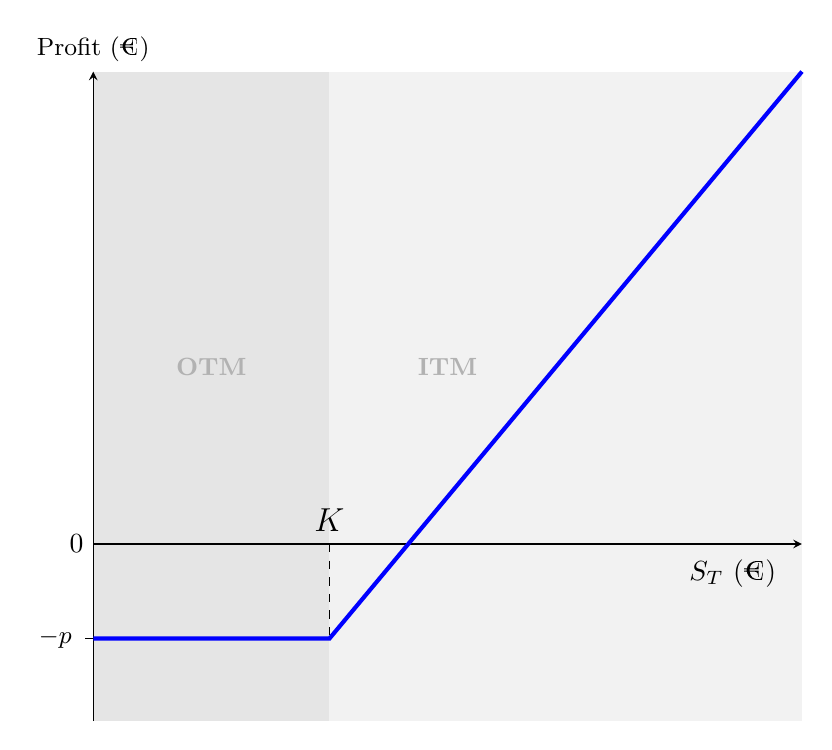
\begin{tikzpicture}[scale=1.5, >=stealth]

        % Shade area to the right of K (extending fully up to x-axis)
        \fill[gray!10] (2,-1.5) -- (6,-1.5) -- (6,4) -- (2,4) -- cycle;

         % Shade area to the left of K (extending fully up to x-axis)
        \fill[gray!20] (0,-1.5) -- (2,-1.5) -- (2,4) -- (0,4) -- cycle;


        % Define axes (extended x-axis)
        \draw[->] (0,0) -- (6,0) node[below,xshift=-25,yshift=-2pt, align=center] {$S_T$ (€)};
        \draw[->] (0,-1.5) -- (0,4) node[above] {\small Profit (€)};
        
        
        % Strike price line
        \draw[dashed] (2,0) -- (2,-0.8) node[above, yshift=35] {\large$K$};
        
        % Payoff function (thicker blue line)
        \draw[line width=1.5pt, blue] (0,-0.8) -- (2,-0.8) -- (6,4);
        
        % Marking zero level
        \node[left] at (0,0) {0};
        
        % Adding the premium annotation
        \draw (-0.07,-0.8) -- (0,-0.8); % Short tick line
        \node[left] at (-0.1,-0.8) {\small $-p$};

        % Add "ITM" label inside the fully shaded area
        \node[gray!60] at (3,1.5) {\small \textbf{ITM}};

        % Add "OTM" label inside the fully shaded area
        \node[gray!60] at (1,1.5) {\small \textbf{OTM}};

    \end{tikzpicture}
    \caption{Profit diagram for the long position in a call option. $K$ = strike price, $S_T$ = spot price, $p$ = premium. The buyer pays a premium to fix a maximum purchase price for the stock at a later point in time. At maturity, as long as $S_T < K$ there is no incentive to exercise the option, and the profit thus equals $-p$. The option is worthless, and is considered out of the money (OTM). When $S_T > K$, the option is in the money (ITM) and is assumed to be exercised as the buyer can now purchase the stock for $K$, immediately sell it for $S_T$, and offset some or all of the premium paid. However, the investment is only profitable once $S_T - K > p$.}
    \label{fig:long_call_payoff}
\end{figure}
\end{center}

The short call position exhibits an inverse profit profile compared to the long position: as long as the option remains OTM, the underwriter retains the full premium as profit, since the investor will not exercise the option. Once the option becomes ITM, the buyer will exercise it, forcing the underwriter to sell the stock at the strike price $K$ despite its higher market value $S_T$. The premium initially offsets this adverse price difference until the breakeven point where $S_T-K=p$, after which the position becomes a loss for the underwriter.~\cref{fig:short_call_payoff} illustrates this position. Continuing with the previous example, this position could be taken by a crude oil producer with conviction that prices will remain below or near the strike price at maturity. The risk borne by the underwriter commands the premium.

Ignoring the premium, the payoff from the long position in a call option is defined as
\begin{equation}
    \max(S_T-K,0)
\label{eq:long_call_payoff}
\end{equation}
as the investor will only exercise when ITM to either profit or offset losses. Consequently, the payoff from the short position is defined as $-\max(S_T-K,0) = \min(K-S_T,0)$ due to the zero-sum nature of the contract.\footnote{For American-style options with the right to early-exercise, the payoff is calculated using $S_\tau$ instead of $S_T$, where $\tau \le T$ is the chosen point of exercise.}\cite{hull2016options}

\begin{center}
\begin{figure}[H]
\centering
    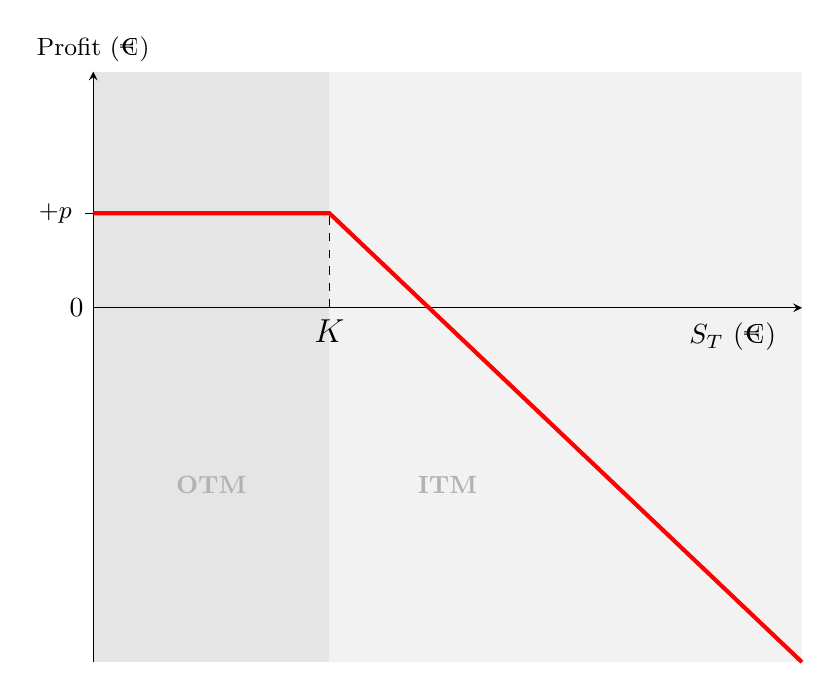
\begin{tikzpicture}[scale=1.5, >=stealth]
        % Create a more balanced diagram by shifting the origin up
        % Define y-range from -3 to +2 instead of -4 to +4
        
        % Shade area to the right of K
        \fill[gray!10] (2,-3) -- (6,-3) -- (6,2) -- (2,2) -- cycle;
        % Shade area to the left of K
        \fill[gray!20] (0,-3) -- (2,-3) -- (2,2) -- (0,2) -- cycle;
        
        % Define axes with shifted x-axis (moved up)
        \draw[->] (0,0) -- (6,0) node[below,xshift=-25,yshift=-2pt, align=center] {$S_T$ (€)};
        \draw[->] (0,-3) -- (0,2) node[above] {\small Profit (€)};
        
        % Strike price line
        \draw[dashed] (2,0) -- (2,0.8) node[below, yshift=-35] {\large$K$};
        
        % Payoff function (thicker red line for short position)
        \draw[line width=1.5pt, red] (0,0.8) -- (2,0.8) -- (6,-3);
        
        % Marking zero level
        \node[left] at (0,0) {0};
        
        % Adding the premium annotation
        \draw (-0.07,0.8) -- (0,0.8); % Short tick line
        \node[left] at (-0.1,0.8) {\small $+p$};
        
        % Add labels inside the shaded areas
        \node[gray!60] at (1,-1.5) {\small \textbf{OTM}};
        \node[gray!60] at (3,-1.5) {\small \textbf{ITM}};
    \end{tikzpicture}
    \caption{Profit diagram for the short position in a call option. $K$ = strike price, $S_T$ = spot price, $p$ = premium. The underwriter receives a premium but is obligated to sell the stock for $K$ at a later time point, should the option be exercised. When $S_T < K$, the option is worthless and considered out of the money (OTM), allowing the underwriter to keep the full premium as profit. When $S_T > K$ and the option is exercised in the money (ITM), the underwriter is forced to sell the stock at the strike price $K$ despite its higher market value $S_T$. The profit decreases linearly as $S_T$ increases, becoming negative once $S_T - K > p$.}
    \label{fig:short_call_payoff}
\end{figure}
\end{center}

For a put option, the investor is willing to pay a premium up front to secure a minimum selling price for the stock at a later time point. They expect the price of the stock to decrease sufficiently to offset this premium. Conversely, the underwriter receives the premium but assumes the obligation to purchase the stock at the strike price $K$, should the option be exercised.~\cref{fig:put_option_payoffs} depicts the profit diagrams of the long and short positions of a put option. A put option is OTM when $S_T > K$ as the investor will not exercise it to sell the stock for a lower price than market value. By the same token, the option is ITM when  $S_T < K$, as the investor can then buy the stock asset at market value and sell it for the strike price \cite{hull2013fundamentals}. Again, being ITM is not sufficient to be profitable - the price difference must be large enough to offset the paid premium. An example use case would be a crude oil supplier forecasting low prices in a year's time and entering the long position to secure a minimum revenue. Again, a premium is paid to hedge against a risk of price swings. The short side would be taken by a market participant who anticipates crude oil prices not to fall enough to offset the received premium.

\begin{figure}[H]
\centering

\begin{subfigure}[t]{0.45\textwidth}
\centering
\resizebox{\linewidth}{!}{%
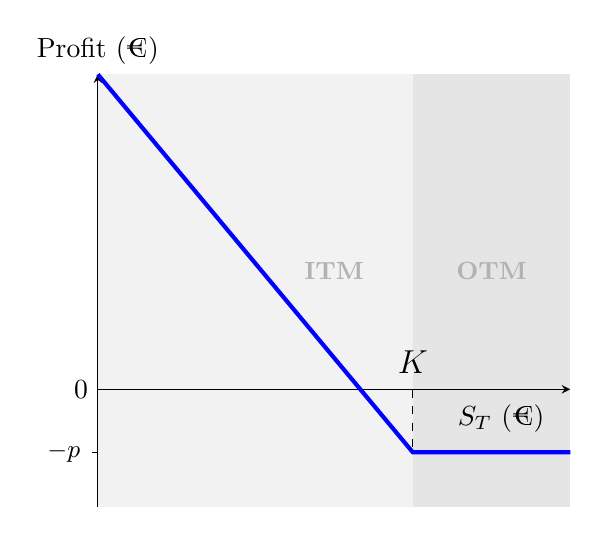
\begin{tikzpicture}[>=stealth]
    \fill[gray!20] (4,-1.5) -- (6,-1.5) -- (6,4) -- (4,4) -- cycle;
    \fill[gray!10] (0,-1.5) -- (4,-1.5) -- (4,4) -- (0,4) -- cycle;
    \draw[->] (0,0) -- (6,0) node[below,xshift=-25,yshift=-2pt] {$S_T$ (€)};
    \draw[->] (0,-1.5) -- (0,4) node[above] {Profit (€)};
    \draw[dashed] (4,0) -- (4,-0.8) node[above,yshift=25] {\large$K$};
    \draw[line width=1.5pt, blue] (0,4) -- (4,-0.8) -- (6,-0.8);
    \node[left] at (0,0) {0};
    \draw (-0.07,-0.8) -- (0,-0.8);
    \node[left] at (-0.1,-0.8) {\small $-p$};
    \node[gray!60] at (3,1.5) {\small \textbf{ITM}};
    \node[gray!60] at (5,1.5) {\small \textbf{OTM}};
\end{tikzpicture}%
}
\caption{Long put option payoff}
\end{subfigure}
\hfill
\begin{subfigure}[t]{0.45\textwidth}
\centering
\resizebox{\linewidth}{!}{%
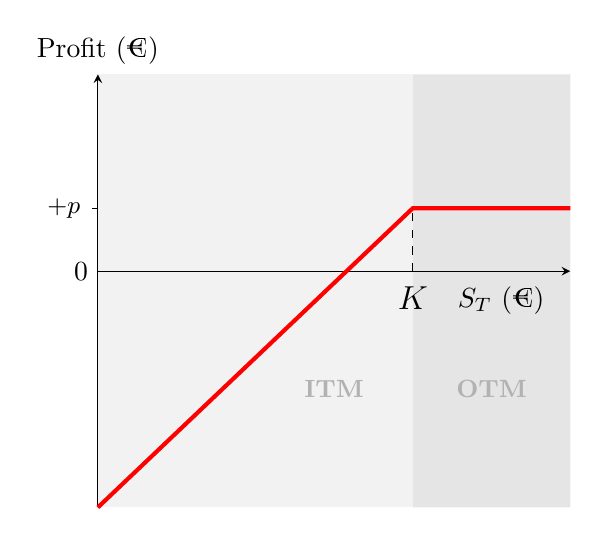
\begin{tikzpicture}[>=stealth]
    \fill[gray!20] (4,-3) -- (6,-3) -- (6,2.5) -- (2,2.5) -- cycle;
    \fill[gray!10] (0,-3) -- (4,-3) -- (4,2.5) -- (0,2.5) -- cycle;
    \draw[->] (0,0) -- (6,0) node[below,xshift=-25,yshift=-2pt] {$S_T$ (€)};
    \draw[->] (0,-3) -- (0,2.5) node[above] {Profit (€)};
    \draw[dashed] (4,0) -- (4,0.8) node[below,yshift=-25] {\large$K$};
    \draw[line width=1.5pt, red] (0,-3) -- (4,0.8) -- (6,0.8);
    \node[left] at (0,0) {0};
    \draw (-0.07,0.8) -- (0,0.8);
    \node[left] at (-0.1,0.8) {\small $+p$};
    \node[gray!60] at (5,-1.5) {\small \textbf{OTM}};
    \node[gray!60] at (3,-1.5) {\small \textbf{ITM}};
\end{tikzpicture}%
}
\caption{Short put option payoff}
\end{subfigure}

\caption{Profit diagrams for long (a) and short (b) positions in a put option. $K$ = strike price, $S_T$ = spot price, $p$ = premium. For the long position, the buyer pays a premium to secure a minimum selling price for the stock at a future time point. When $S_T < K$ the option is in the money (ITM) and would be exercised, as the underwriter is forced to buy the stock for $K$ despite its lower market value $S_T$. When $S_T > K$ the option is out of the money (OTM) with no incentive to exercise, resulting in a loss $-p$. For the short position, the underwriter receives the premium but assumes the obligation to purchase the stock at $K$, should the option be exercised. The underwriter profits fully when the option remains OTM, but faces decreasing profits when ITM as the spot price decreases. The position becomes unprofitable once $K-S_T > p$.}
\label{fig:put_option_payoffs}
\end{figure}

The payoff from the long position in a put option is defined as
\begin{equation}
    \max(K-S_T,0)
\label{eq:long_put_payoff}
\end{equation}
as being ITM now means $K > S_T$. Conversely, the payoff in the corresponding short position is $-\max(K-S_T,0) = \min(S_T-K,0)$ \cite{hull2016options}.

The long position in any option contract is never obligated to exercise, and the loss is therefore limited to the premium paid. On the other hand, the underwriter is always obligated to engage in a disadvantageous trade with the buyer. Additionally, since underlying asset prices have no theoretical upper bound but are limited to non-negative values, the short call position faces potentially unlimited losses. \cref{tab:options_table} aggregates information about the extreme-case profit and loss incurred from the different option types and positions.

\begin{table}[!htb]
\centering
\caption{Extreme-case upside and downside potential for different option positions. $p$ = premium paid or received, $K$ = strike price. The long position in a call option has unlimited upside potential due to theoretically unbounded underlying asset prices, with losses limited to the premium paid. The corresponding short position mirrors this behavior with unlimited downside risk. Put options have bounded payoffs as asset prices cannot fall below zero. The maximum gain for a long put position is $K-p$ when the spot price reaches zero, and the maximum loss for the corresponding short position is $-(K-p)$.}\label{tab:options_table}
\begin{tabular}{|l|p{5cm}|p{5cm}|}
\hline
\textbf{} & \textbf{Call Option} & \textbf{Put Option} \\
\hline
\textbf{Long} & \textbf{Maximum Gain:} $+\infty$
\newline \textbf{Maximum Loss:} $-p$ & \textbf{Maximum Gain:} $K-p$
\newline \textbf{Maximum Loss:} $-p$ \\
\hline
\textbf{Short} & \textbf{Maximum Gain:} $+p$
\newline \textbf{Maximum Loss:} $-\infty$ & \textbf{Maximum Gain:} $+p$
\newline \textbf{Maximum Loss:} $-(K-p)$ \\
\hline
\end{tabular}
\end{table}

The objective of pricing models is to find the so-called fair value of the option~$p$. Although market prices form through the dynamic interaction of buyers and sellers, they are still largely anchored by theoretical pricing frameworks. These models provide a rational foundation for valuing derivatives based on mathematical and economic theory. While real-world prices may show short-term deviations, markets tend to converge toward theoretically justified values over time, as persistent mispricing creates exploitable opportunities. The theoretical fair value serves as a crucial reference point that informs trading decisions and risk management strategies.

\subsection{Price Determinants}

Hull et al.\ \cite{hull2013fundamentals} define six factors influencing the price of the option. While these factors typically serve as variables in pricing models, their effects can be intuitively understood even without formal mathematical frameworks. When analyzing a factor's impact, it is usually done in a ``ceteris paribus'' manner. In practice, however, this isolation rarely occurs, as markets quickly incorporate all available information into prices \cite{fama1970efficient}, causing interrelated changes among the factors themselves. For clarity, the following analysis considers the long position, though the same reasoning applies symmetrically to the short position, as both sides value the same option.

The stock price relative to the strike price is perhaps the most obvious factor. The effect on the payoff is thoroughly explained in \cref{subsec:payoffs}, and the price naturally increases with the payoff. Thus, the price of a call option increases with the stock price, while the inverse relationship is observed for a put option.

Volatility, a statistical measure of the variation in asset prices over a specific time period, has a positive effect on both call and put options. This positive relationship can be motivated by the limited downside -- unlimited upside nature of options (~\ref{fig:optiontable}). Higher stock price volatility increases the probability of significant movements, making it more likely the option will move ITM. The benefit is especially pronounced for OTM positions, where substantial price movement is needed to avoid expiring worthless, but holds for ITM positions as well. In the latter case, the unlimited potential for becoming even deeper ITM outweighs the limited downside risk of moving OTM.

Time to maturity has a more complex relationship with the price, and depends on both the option style and the context. For American options with possibility of early exercise, it makes sense that an expiration date further in the future leads to more opportunity for favorable movements in the stock price, thereby commanding a higher price. This time value argument is similar to that made for volatility, where the asymmetric payoff structure means additional potential for gain typically outweighs the risk of further losses. While this time value argument also holds for European options, the lack of early-exercise ability introduces complications. Hull et al.\ \cite{hull2013fundamentals} identify specific scenarios where American options derive significant additional value from the early exercise privilege. One example is when a future dividend payment to shareholders is expected, which theoretically decreases the share price and thereby the value of the corresponding call option. Similarly, a put option might be more valuable with a shorter time to maturity in the case of a very deep ITM position, such as when the underlying company has filed for bankruptcy. The option will almost certainly expire ITM, and thus by the \emph{time value of money} \textbf{(should I explain this in a footnote in greater detail?)} principle this cash flow is worth more the earlier it is received \cite{berk2007corporate}.

The risk-free rate represents the return on investment one can expect from a so-called risk-free investment, typically government-backed treasury securities. It serves as a benchmark against which investors compare expected returns of riskier investments. An increase in the risk-free rate typically leads to investors demanding higher returns across all risk levels. In option pricing, the risk-free rate primarily affects the time value component through the discounting of future cash flows. For a call option, a higher risk-free rate reduces the present value of the strike price that will be paid in the future\footnote{The present value of a future cash flow is calculated by discounting it using an appropriate rate. This rate reflects both the time value of money and opportunity cost. The risk-free rate represents the minimum discount rate, as it corresponds to the return available from risk-free investments. For risky cash flows, an additional risk premium is added to this base rate.}. This economic advantage for the buyer is reflected in the market through a higher option price. Conversely, for put options, a higher risk-free rate decreases the present value of the strike price to be received in the future, reducing the economic benefit to the holder and thereby decreasing the option's price. In practice, however, interest rates impact stock prices as well, making this relationship more complex when applied to actual markets.

The final determinant considers the dividend policy of the underlying company. Theoretically, a company's share price is reduced by the dividend amount on the ex-dividend date, as this cash is directly distributed from the company's assets to shareholders \cite{modigliani1958cost}. For call options, expected dividends decrease value because they reduce the expected future price of the stock without providing any benefit to the option buyer. Conversely, put options increase in value with higher expected dividends, as they decrease the value of the stock. This dividend effect is particularly significant for longer-dated options, where multiple dividend payments may occur before expiration, and for options near the money, where the dividend-induced price movement can meaningfully change the moneyness of the option.

\subsection{No-Arbitrage Pricing and Risk-Neutral Valuation}\label{sec:risk-neutral-theory}
Previously, all main "ingredients" for the pricing formulas were introduced. This section outlines the foundational theoretical framework that underpins all option pricing models, bringing us one step closer to formulating the models to be GPU-accelerated. In line with the thesis scope, the focus will be on intuition rather than mathematical rigor. Avid readers are encouraged to explore the references in greater detail \cite{hull2016options, gisiger2010risk, tham2001risk}. The assumptions presented in \cref{subsec:payoffs} continue to hold, as will the referral of the underlying asset as the stock. The setup considers European-style options, but in this single-period setting, the results are equally valid for American options, as early exercise provides no advantage.

A natural starting point is to consider how other financial assets are valued. The theoretical value of an asset is commonly understood as the discounted sum of all future cash flows it produces. Under uncertainty -- as is the case of all risky assets -- a standard approach would be to discount the \emph{expected value} of these cash flows, which represents a theoretical long-term average of the returns \textbf{(basic math and financial theory, do I need src for this?)}. Calculating this expected value, however, requires defining a set of possible outcomes and assigning probabilities to each. This is a fundamental limitation of pricing models, as the estimates are often questionable and, at least in part, subjective. Nonetheless, starting out with a simplistic model will lead to interesting and useful revelations that can be expanded on.

The \emph{no-arbitrage principle} is the essential assumption for what is to come. Arbitrage describes the act of simultaneous buying and selling of the same asset in different markets to make risk-free profit off price differences. Imagine the price of tomatoes being higher in one of two neighboring towns. Perhaps the tomato farmers were really successful in town A this year, and the increased supply dropped the prices somewhat. This information has not yet been priced into the tomatoes in town B. The astute tradesman could then buy tomatoes in town A and immediately sell them in town B to pocket the difference, without taking any position on future tomato price movements. This, again, assumes ideal conditions, like enough liquidity to always be able to both buy and sell, as well as ignoring friction costs like transportation. The idea behind our assumption is that this strategy ultimately is self-eliminating: as the tradesman continues to introduce more tomatoes to the total supply in town B they will drive the price down until an equilibrium has been reached. Other people may take notice and decide to adopt the same strategy, eliminating the opportunity even faster. The information about the larger supply in town A has now been priced into the tomatoes in town B. This example is not too far-fetched from reality. Modern digital markets do not perfectly adhere to the assumptions laid out above, and short-term arbitrage opportunities can exist. Nevertheless, as sophisticated market participants exploit these inefficiencies they quickly disappear due to subsequent price corrections. Thus, the no-arbitrage principle is a reasonable assumption, at least over longer time periods. If our pricing methodology is based on summing future cash flows, it logically follows that in absence of arbitrage opportunities two assets producing the same cash flows must be priced equally \cite{hull2016options,wilmott2013paul}.

If it is possible to find an existing asset with identical future cash flows to those of the option, and whose price is already known, then by the no-arbitrage principle, the price of that asset should theoretically equal the price of the option. Hull~et~al.~\cite{hull2013fundamentals} consider a one-step model as the simplest framework to apply this idea. In this discrete-time model, we consider the stock price evolution over a single period. Let $S_0$ denote the current stock price, and let $f$ be the current price of an option on one share, with time $T$ to maturity. The stock price is assumed to move to one of two possible future values: $S_0u$ or $S_0d$ ($u>1$, $d<1$). These correspond to the option payoffs $f_u$ and $f_d$, respectively. \cref{fig:oneperiodbinom} visualizes the model setup. This restriction makes it possible to construct a so-called \emph{replicating portfolio} that perfectly matches the option's payoff in both states. This portfolio consists of $\Delta$ shares of the stock, as well as $B$ amount of a risk-free asset (e.g., a savings account) growing at the risk-free rate $r$. After time $T$, the portfolio will take on one of two values, depending on whether the stock price increased or decreased. By equating the value of the portfolio in each case with the corresponding option payoff, one obtains a system of two equations and two unknowns, $\Delta$ and $B$.

\begin{equation*}
\begin{cases}
    \Delta (S_0u) + B(1+r) = f_u\\
    \Delta (S_0d) + B(1+r) = f_d
\end{cases}
\end{equation*}
Solving for these variables yields
\begin{equation*}
\begin{cases}
    \Delta = \frac{f_u - f_d}{S_0(u-d)}\\
    B = \frac{f_du-f_ud}{(u-d)(1+r)}
\end{cases}
\end{equation*}

It is evidently possible to construct a portfolio with identical payoff structure as the option itself, according to

\begin{equation}
     \frac{f_u - f_d}{S_0(u-d)} S_0 + \frac{f_du-f_ud}{(u-d)(1+r)}
\label{eq:replicating-portfolio}
\end{equation}

Under the no-arbitrage principle, the price of the option must thus equal the price of constructing the replicating portfolio, i.e., buying $\Delta$ shares and investing $B$ in a risk-free asset. Otherwise, one could buy the cheaper alternative while selling the more expensive to obtain a risk-free profit. A negative $\Delta$ implies shorting the underlying asset, and a negative $B$ implies borrowing money at the risk-free rate instead of lending (saving) it.
\begin{figure}[htbp]
    \centering
    \begin{tikzpicture}[
        scale=1.5,
        >=stealth,
        every node/.style={font=\normalsize}
    ]
    
    % Stock price nodes
    \node (S0) at (0,0) {$S_0$};
    \node (Su) at (4,2) {$S_0u$};
    \node (Sd) at (4,-2) {$S_0d$};
    
    % Add option payoffs directly under stock prices
    \node at (0,-0.5) {$f$};
    \node at (4,1.5) {$f_u$};
    \node at (4,-2.5) {$f_d$};
    
    % Edges without probabilities
    \draw[->, thick] (S0) -- (Su);
    \draw[->, thick] (S0) -- (Sd);
    
    % Timeline moved closer to the lattice
    \draw[->, thick] (0,-3) -- (4,-3);
    \node at (0,-3) [below] {$t=0$};
    \node at (4,-3) [below] {$t=T$};
    
    \end{tikzpicture}
    \caption{One-period binomial model showing stock price evolution and corresponding option payoffs. The stock price moves from $S_0$ to either $S_0u$ or $S_0d$, with corresponding option values $f_u$ and $f_d$. The replicating portfolio approach determines the option price $f$ without requiring knowledge of the actual probabilities of up or down movements.}
    \label{fig:oneperiodbinom}
\end{figure}

The derivation assumed neither a call nor a put option, and works therefore as a pricing model for any European option. A more interesting observation, however, is the fact that this pricing approach contains no information about the expected return of the stock, or the probability with which it will increase or decrease in value. The authors motivate this intuitively by the fact that such expectations are already reflected in the stock price itself, and need not be explicitly accounted for when pricing the derivative. The option is priced relative to the underlying stock.

This also leads to the fundamental concept of \emph{risk-neutral} valuation. \cref{eq:replicating-portfolio} can be rewritten as

\begin{equation*}
     \frac{1}{1+r}\left(f_u\frac{(1+r)-d}{u-d}+f_d\frac{u-(1+r)}{u-d}\right),
\end{equation*}

where the weights $\tilde{p} := \frac{(1+r)-d}{u-d}$ and $\tilde{q} := \frac{u-(1+r)}{u-d}$ sum to one and lie between 0 and 1 under the no-arbitrage condition $d \leq 1+r \leq u$. These are called risk-neutral probabilities, and the option price can thus be calculated as the expected value of its payoff using the risk-neutral probabilities, discounted at the risk-free rate

\begin{equation}
     \frac{1}{1+r}(f_u\cdot \tilde p + f_d \cdot (1-\tilde p)).
\label{eq:risk-neutral-expectancy}
\end{equation}

While there exist many misconceptions about risk-neutral valuation, it can simply be thought of as an algebraic reformulation of the problem into a more familiar version of discounting expected future cash flows. The risk-neutral probabilities are not predictions of any real-life events. They are mathematical weights that look and behave like probabilities, and produce the same price as the replicating portfolio while maintaining the no-arbitrage assumption. The term risk-neutral probability stems from the fact that the reformulation discounts by the risk-free rate, resembling how a risk-neutral investor would discount cash flows. This elegant reformulation enables the use of more tools from probability theory, and elements of it will be found in all of the models to be introduced later. The full derivation of this reformulation is provided in \cref{appendix:risk_neutral_derivation}. \cite{gisiger2010risk, tham2001risk}

\section{GPU and Parallel Computing}
The graphics processing unit (GPU) is a processor specifically tailored for graphics-related computation. Starting in the 1980s, the demand for 2D and 3D graphics-based consumer software, mainly driven by video games, surged. The computations entailed performing a large amount of floating-point operations per seconds (FLOPS) associated with graphics, like shading and rasterization~\cite{sanders2010cuda, kirk2016programming}. Front-runners of delivering affordable graphics computing capabilities included NVIDIA and ATI Technologies (later acquired by AMD)~\cite{sanders2010cuda}.

Hennessy and Patterson \cite{hennessy2011computer} loosely define \emph{latency} as the time between the start and completion of a single event, and \emph{throughput} as the total amount of work performed in a given time. These metrics (and specific variants thereof) are widely used in computing performance contexts. While both central processing units (CPUs) and GPUs have seen performance improvements in both metrics, the authors show that relative throughput improvements have surpassed relative latency improvements. This is not unreasonable: Increasing throughput is mainly a matter of providing more of the same already available resource. Latency improvements have, on the other hand, already reached closer to the theoretical limits imposed by the laws of physics \cite{hennessy2011computer} \cite{sanders2010cuda}. Suomela's summary of statistics on trends for both clock speed and instruction latencies corroborate these claims \cite{suomela_ppc}.

This, in combination with the fact that graphics-related calculations are well-structured for concurrency exploitation (covered in \cref{subsec:parallell}), led to the evolution towards the exceptionally throughput-optimized GPU architectures of the modern age. At the same time, there grew an increasing interest in the utilization of these parallel computing capabilities for other purposes. However, these advances alone were insufficient in unlocking the potential for so-called general-purpose GPU (GPGPU) programming, as the hardware lacked the flexibility needed for general-purpose computing, and no GPGPU programming models and tools were readily available. The initial graphics-intended hardware and software ecosystems effectively forced developers to mask their problems as those found in the graphics domain \cite{sanders2010cuda, kirk2016programming}. Only after advances in these areas could GPGPU programming truly flourish. In 2007, NVIDIA released \emph{CUDA (Compute Unified Device Architecture)}, a software abstraction layer that greatly removed earlier restrictions in favor of GPGPU-programming. The hardware was now directly accessible without considering graphics-related interfaces, and writing CUDA applications was possible as a simple extension layer on top of familiar C/C++. Today, GPGPU applications are found in a wide variety of fields, including computational finance \cite{sanders2010cuda, kirk2016programming}.

\subsection{CPU and GPU Architecture}
 \cref{fig:CPUandGPU} represents a simple model of a modern CPU and GPU. The CPU portion is based on the writings of Stallings~\cite{stallings2011operating}, while the GPU portion is derived from both the work of Kirk and Hwu~\cite{kirk2016programming} and the CUDA C++ Programming Guide by NVIDIA~\cite{cuda2025guide}. 

 The arithmetic logic unit (ALU) is responsible for performing bitwise operations on data, registers (not visible in figure) store memory addresses, instructions, and data to operate on, and additional support components for control of flow and communication with the external environment. The CPU operates in a loop of two-staged fetch-execute instruction cycles, where an instruction is first loaded into a register. After this, the instruction is executed, which in practice means either data processing, data transfer, or control logic related to the instruction sequence. This loop continues until the program terminates, e.g. from finishing or halting due to an error, or due to an interruption by another module~\cite{stallings2011operating}.

CPUs have evolved to improve performance by leveraging various forms of parallelism. Instruction-level parallelism (ILP) refers to a set of techniques that allow a processor to execute multiple independent instructions simultaneously or in overlapping stages. Examples include instruction pipelining, superscalar execution, and out-of-order execution. Additional techniques like branch prediction and speculative execution support ILP by keeping the pipeline filled \cite{hennessy2011computer, suomela_ppc}.

Modern CPUs also possess \emph{single instruction multiple data} (SIMD) capabilities through large vector registers capable of storing multiples of the same data type, and instructions that can operate on these at once. And to top it off, most modern processors are multi-core, meaning they literally contain multiple instances of the main aforementioned components for use. This enables a higher, thread-level parallelism (TLP), where a \emph{thread} -- an independent sequence of instructions that can be scheduled and executed \cite{stallings2011operating} -- can run on each core simultaneously \cite{hennessy2011computer, suomela_ppc}. Nonetheless, CPUs remain fundamentally optimized for low-latency sequential execution and control flow, rather than for maximizing throughput.

\begin{figure}[htbp]
  \centering
  \begin{tikzpicture}
    \node[anchor=south west, inner sep=0] (image) at (0,0) {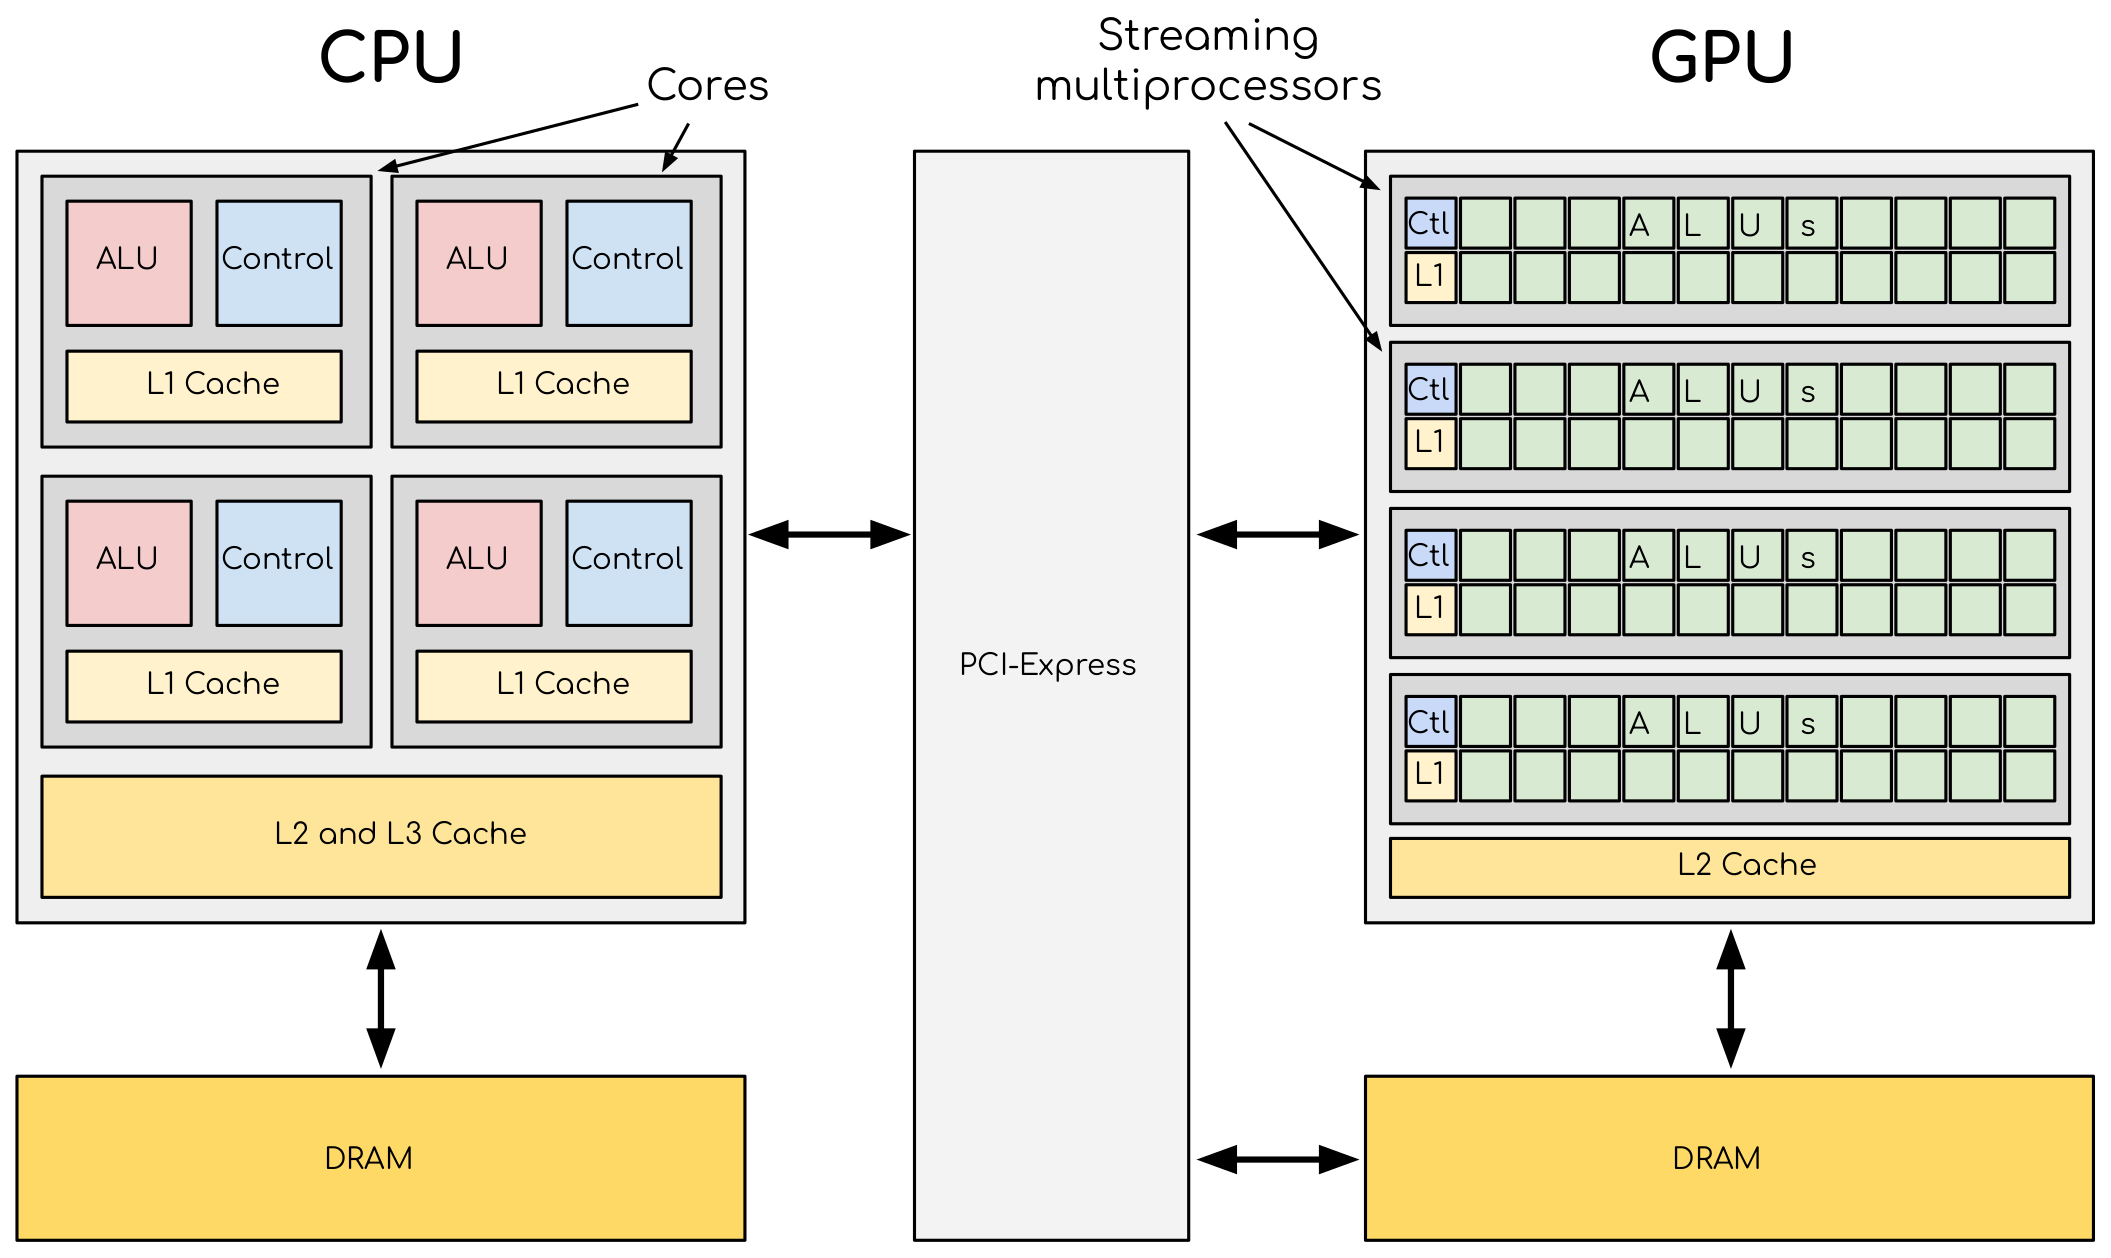
\includegraphics[width=\textwidth]{External Images/CPUandGPU.png}};
    \begin{scope}[x={(image.south east)}, y={(image.north west)}]
      % Adjusted positions for the Shared Memory blocks
      \foreach \y in {0.806, 0.676, 0.545, 0.413} {
        \draw[fill=orange!80!black] (0.692,\y-0.047) rectangle (0.74,\y+0.035);
        \node[font=\sffamily\tiny, align=center, scale=0.9] at (0.716, \y-0.006) {Shared\\Memory};
      }
    \end{scope}
  \end{tikzpicture}
  \caption{Simple diagrams of modern multi-core CPU and GPU architectures, showcasing their main respective components. Each CPU core contains an arithmetic logic unit (ALU) for performing bitwise operations and a control unit for handling program flow. Hierarchical (L1-L3) on-chip cache memory minimizes data transfer bottlenecks between the RAM and the cores. On the GPU, streaming multiprocessors correspond to cores, and their design clearly emphasizes parallel computing power over control and latency optimization. The PCI-Express serves as a communication interface between the processors. Adapted from material by ENCCS, licensed under CC-BY 4.0 \cite{enccs2025gpu}.}
  \label{fig:cpu-gpu-architecture}
\end{figure}


In contrast, while lacking many of the sophistication that makes the CPU excel at sequential and control-heavy tasks, the GPU fits in more raw computation power for a massively throughput-optimized architecture that excels at parallel numerical computation. The term single instruction multiple thread (SIMT) is often used to describe GPU computation, as the concurrency is enabled on thread-level by a massive amount of threads executing the same instruction in parallel, as opposed to single-threaded computation using SIMD, ILP, or multi-threading on a comparatively few cores \cite{cuda2025guide}. A modern GPU contains independent \emph{streaming multiprocessors} (SM), which can be considered as a group of many processing units sharing some control units and memory. Threads are grouped into units of 32, called \emph{warps}, which generally execute in lock-step on a single SM.\footnote{Since the release of the NVIDIA Volta architecture in 2017, GPUs support individual threads within a warp to follow divergent control flow. This allows greater flexibility for algorithms with complex control flow or thread-level synchronization \cite{cuda2025guide}. However, full parallelism is only maintained when threads execute the same instruction. Divergence still reduces efficiency as execution becomes serialized across paths.}, i.e. simultaneous execution on their respective data. Similarly to a multi-core CPU, all SMs share a higher-latency RAM, and are individually allocated smaller but faster cache memory for minimizing data transfer bottlenecks . Additionally, each SM contains \emph{shared memory}, a low-latency programmer-controlled memory region for inter-thread communication within a streaming multiprocessor \cite{sanders2010cuda, cuda2025guide, kirk2016programming}.

\subsection{Parallel Computing Fundamentals and GPU suitability}\label{subsec:parallell}

A theoretical framework is greatly helpful in analyzing parallelism opportunities and limitations. This chapter introduces key concepts for assessing algorithm structure, theoretical speedup limits, and common pitfalls.

Kirk et al. \cite{kirk2016programming} denote two forms of parallelism: data parallelism and task parallelism. The former denotes performing the same operations in parallel on different data, while the latter means performing multiple different tasks simultaneously. A simple example of data parallelism is vector addition, where each respective component in vector A is added to its corresponding component in vector B. As per the authors, data parallelism is more abundant, especially in the modern age as programs make use of increasingly large data sets. The SIMT architecture of GPUs also favors data parallelism over task parallelism, as it is precisely optimized for lock-step execution of a single instruction on different data elements, as opposed to fine-grain control flow. This stems from the nature of graphics-related computation, the GPUs original purpose, where color values quickly had to be updated on many thousands of pixels at the same time \cite{sanders2010cuda}. The authors do not dismiss task parallelism completely, suggesting it often can be exploited by partitioning and identifying smaller independent sub-tasks of a program \cite{kirk2016programming}.

Acar \cite{acar2016parallel} provides a framework for a more formal analysis of parallel algorithms. The algorithm is depicted as a directed acyclic graph (DAG), whose nodes represent executions of individual instructions, and whose edges represent instruction dependencies. The DAG can be thought of as a Hasse diagram that depicts a partial ordering of these instructions under the relation "must execute before". Acar sets the maximum node \emph{out-degree} and \emph{in-degree}\footnote{The number of edges extending out from or into a node.} to two, representing the cases of spawning a new thread and synchronizing the result from two threads. \cref{fig:DAG-algo} depicts a DAG representation of an algorithm.

\begin{figure}[h]
\centering
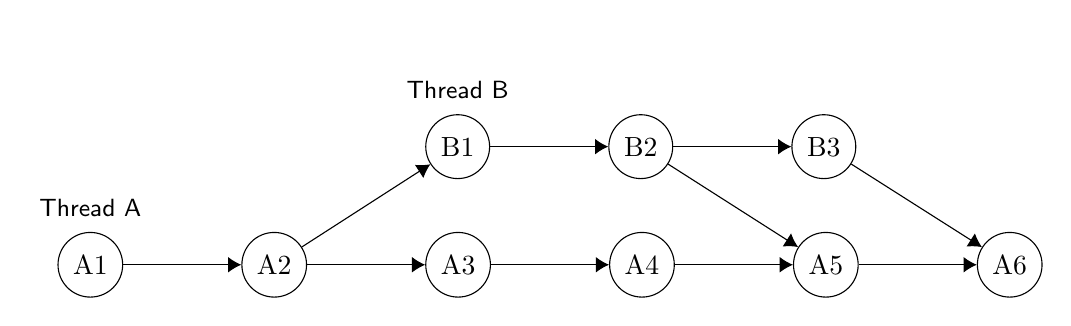
\begin{tikzpicture}[
    node distance=1.5cm and 1.5cm,
    every node/.style={draw, circle, minimum size=8mm},
    every edge/.style={draw, -{Latex[width=2mm]}},
    threadlabel/.style={font=\sffamily\small, draw=none, fill=none},
]

% Nodes
\node (A1) {A1};
\node[right=of A1] (A2) {A2};
\node[right=1.5cm and 1.5cm of A2, yshift=1.5cm] (B1) {B1};
\node[right=of A2] (A3) {A3};
\node[right=of B1] (B2) {B2};
\node[right=of A3] (A4) {A4};
\node[right=of A4] (A5) {A5};
\node[right=of B2] (B3) {B3};
\node[right=of A5] (A6) {A6};

% Edges
\draw (A1) edge (A2);
\draw (A2) edge (B1);
\draw (A2) edge (A3);
\draw (B1) edge (B2);
\draw (A3) edge (A4);
\draw (A4) edge (A5);
\draw (B2) edge (A5);
\draw (B2) edge (B3);
\draw (A5) edge (A6);
\draw (B3) edge (A6);

% Plain text thread labels (no bubbles)
\node[threadlabel, above=-0.5cm of B1] {Thread B};
\node[threadlabel, above=-0.5cm of A1] {Thread A};

\end{tikzpicture}
\caption{Directed acyclic graph (DAG) representation of a parallel algorithm. The nodes represent individual instructions and the edges represent instruction dependencies that form the order of execution. At node A2, a new thread is spawned, after which both execute independent instruction sequences in parallel. The thread results synchronize at nodes A5 and A6, but thread B terminates only at the latter. DAG representations help visualize the algorithm structure and where parallelism can be utilized on independent computation paths.}
\label{fig:DAG-algo}
\end{figure}

Using these graphs, Acar \cite{acar2016parallel} defines the \emph{work} of an algorithm as the total number of nodes in the DAG, and \emph{span} as the length of its longest path. Alternatively, assuming each instruction takes a unit of time and no overhead cost of thread management, one can think of the work as the sequential run-time on a single processor $T_1$, and span as the run-time on an idealized infinite-processor machine $T_{\infty}$. For instance, the DAG presented in \cref{fig:DAG-algo} contains nine units of work but the span only six units. It is now possible to define two lower bounds on algorithm run-time on a p-processor machine $T_p$:

\paragraph{Span-limited lower bound $T_p \geq T_\infty$}: No matter the number of processors available, the execution cannot be faster than the longest dependency chain in the DAG. This illustrates the role of algorithm structure in parallelization potential, and motivates the effort to restructure algorithms to minimize span and other dependency chains.

\paragraph{Work-limited lower bound $T_p \geq T_1/p$}: $p$ processors can perform at most $p$ operations in parallel, even if there are no dependencies. This highlights hardware constraints.

Furthermore, the author demonstrates how an upper bound on the runtime can be obtained based on \emph{Brent's theorem}. For both level-by-level and greedy scheduling\footnote{level-by-level scheduling assigns nodes to processors by a level-order traversal of the DAG. This can leave processors idle if the amount of nodes per level does not evenly divide the amount of processors. In contrast, greedy scheduling minimizes processor idling by immediately assigning available nodes to them.}, the upper bound is within a factor 2 of the lower bound, underlining once more the importance of minimizing span and providing enough resources to divide the work \cite{acar2016parallel}. In practice, runtime analysis is often more complex due to factors such as varying instruction latencies, parallelization overhead, and synchronization and shared resource contention.


\clearpage

\section{GPU Acceleration of the Cox-Ross-Rubinstein Binomial Model} \label{sec:gpu-crr}

\subsection{The Cox-Ross-Rubinstein Model}

The Cox-Ross-Rubinstein (CRR) model extends the single-period framework into a multi-period setting, providing a more realistic model of asset price evolution over time. The model maintains the same assumptions as the single-period case: discrete time periods and constant multiplicative factors $u$ and $d$ for price movements. Over multiple periods, this creates a binomial lattice of possible price paths. This lattice expands outward from the initial stock price, generating multiple possible final states for both the stock and the corresponding option payoff. The CRR model solves for the initial option price using backward induction. Starting at the terminal nodes, where option payoffs are calculated using \cref{eq:long_call_payoff,eq:long_put_payoff}, the algorithm moves backward through the lattice. Each interior node is treated as a one-period binomial problem, and the option value is calculated using \cref{eq:risk-neutral-expectancy}. \cref{fig:crr-twoperiod} visualizes a two-period lattice, but this can be extended to an arbitrary number of periods. \cite{cox1979option}

\begin{figure}[tbp]
    \centering
    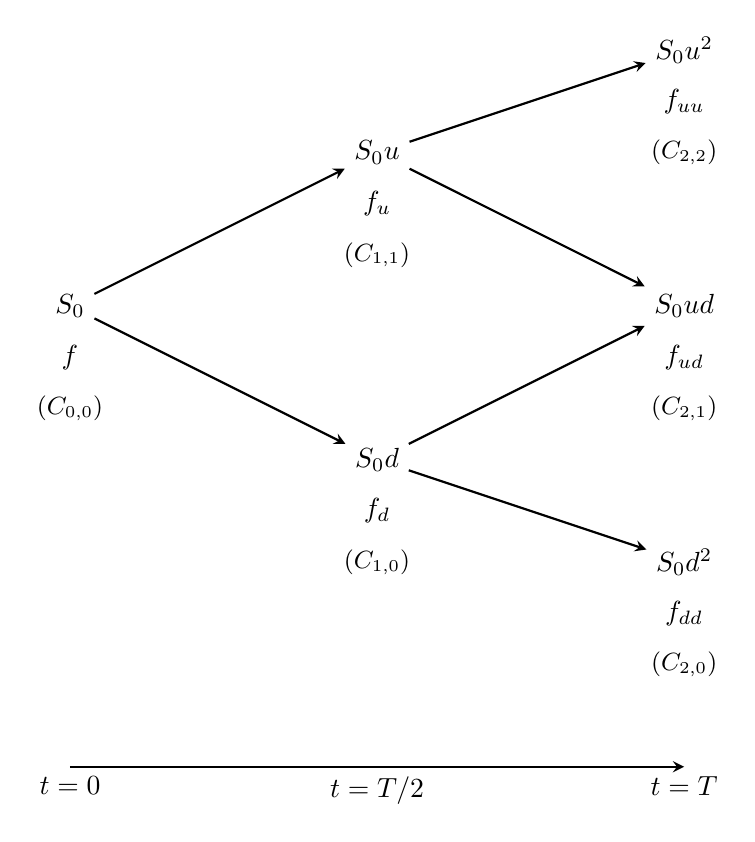
\begin{tikzpicture}[
        scale=1.3,
        >=stealth,
        every node/.style={font=\normalsize}
    ]
    
    % T = 0
    \node (S0) at (0,0) {$S_0$};
    \node at (0,-0.5) {$f$};
    \node at (0,-1.0) {\small $(C_{0,0})$};  % Moved down
    
    % T = 1
    \node (Su) at (3,1.5) {$S_0u$};
    \node at (3,1) {$f_u$};
    \node at (3,0.5) {\small $(C_{1,1})$};   % Moved down
    \node (Sd) at (3,-1.5) {$S_0d$};
    \node at (3,-2) {$f_d$};
    \node at (3,-2.5) {\small $(C_{1,0})$};  % Moved down
    
    % T = 2
    \node (Suu) at (6,2.5) {$S_0u^2$};
    \node at (6,2) {$f_{uu}$};
    \node at (6,1.5) {\small $(C_{2,2})$};   % Moved down
    \node (Sud) at (6,0) {$S_0ud$};
    \node at (6,-0.5) {$f_{ud}$};
    \node at (6,-1.0) {\small $(C_{2,1})$};  % Moved down
    \node (Sdd) at (6,-2.5) {$S_0d^2$};
    \node at (6,-3) {$f_{dd}$};
    \node at (6,-3.5) {\small $(C_{2,0})$};  % Moved down
    
    % Forward edges (stock price evolution)
    \draw[->, thick] (S0) -- (Su);
    \draw[->, thick] (S0) -- (Sd);
    \draw[->, thick] (Su) -- (Suu);
    \draw[->, thick] (Su) -- (Sud);
    \draw[->, thick] (Sd) -- (Sud);
    \draw[->, thick] (Sd) -- (Sdd);
    
    % Timeline
    \draw[->, thick] (0,-4.5) -- (6,-4.5);  % Moved timeline down slightly too
    \node at (0,-4.5) [below] {$t=0$};
    \node at (3,-4.5) [below] {$t=T/2$};
    \node at (6,-4.5) [below] {$t=T$};
    
    \end{tikzpicture}
        \caption{Two-period binomial lattice. Stock prices evolve forward through time, creating an expanding set of possible outcomes. Option payoffs are calculated at the terminal nodes, after which option values at interior nodes can be calculated using \cref{eq:risk-neutral-expectancy}. The symbols $C_{i,j}$ represent the algorithmic notation for the option values, where $i$ is the time point and $j$ is the number of up-ticks the stock price has moved. }
    \label{fig:crr-twoperiod}
\end{figure}

A detail not yet discussed is the choice of the factors $u$ and $d$. The authors of the original paper have defined $u = e^{\sigma\sqrt{T/n}}$ and $d = e^{-\sigma\sqrt{T/n}}$, where $\sigma$ is the annualized volatility (e.g. estimated from historical data) of the log-return of the asset, $T$ is the total time in years, and $n$ is the number of time periods. This is useful for several reasons: firstly, it allows for the model to converge to the famous Black-Scholes-Merton (BSM) model as $n \rightarrow \infty$. Secondly, the lattice recombines for all permutations of a price path. This ensures computational feasibility as the number of states grows linearly instead of exponentially. Another detail to note is that the discount rate used in the period calculations must be adjusted such that it yields the same return as the initial risk-free rate used in the one-period example. A continuous compounding rate $e^{rT/n}$ is often used in lieu of the discrete version. \cite{cox1979option} \cite{hull2013fundamentals}

The implementation of the CRR model comprises three steps: first, compute the price of the underlying at all the terminal nodes. Then, calculate the corresponding option payoffs for the terminal nodes. Finally, backtrack the lattice to compute the option values at nodes in the previous period, working towards the initial node. The following pseudocode is based on the Python implementation by Jonathon Emerick \cite{thequantpy2024github}. Let $S_0$ be the initial stock price and $n$ the number of periods. The nodes of the recombining lattice can be expressed in terms of indices $i$ and $j$, where $0 \leq i \leq n$ are points in time, ranging from the start to maturity, and $0 \le j \le i$ are the nodes at time point $i$ based on the number of up-ticks $j$ the stock price has moved. In other words, the stock price at each node is defined as $S_{i,j} = S_0u^jd^{i-j}$. In the same manner, $C_{i,j}$ represents the option price at the corresponding node. The option price  $C_{0,0}$ is calculated according to \cref{alg:crr-european}.

\begin{algorithm}
\caption{CRR European Option Pricing}
\label{alg:crr-european}
\textbf{Data:} $S_0$ (initial stock price), $K$ (strike price), $T$ (time to maturity), $r$ (risk-free rate), $n$ (periods), $\sigma$ (volatility), type $\in \{\text{CALL}, \text{PUT}\}$\\
\textbf{Result:} Option price at $t=0$\\
$\Delta t \gets T/n$\;
$u \gets e^{\sigma\sqrt{\Delta t}}$\;
$d \gets 1/u$\;
$disc \gets e^{-r\Delta t}$\;
$p \gets (e^{r\Delta t} - d)/(u - d)$\;
/* Compute stock prices at terminal nodes */\\
Initialize $S[0..n]$\;
$S[0] \gets S_0 \cdot d^n$\;
\For{$j \gets 1$ \KwTo $n$}{
    $S[j] \gets S[j-1] \cdot u/d$\;
}
/* Compute option payoffs at terminal nodes */\\
Initialize $C[0..n]$\;
\For{$j \gets 0$ \KwTo $n$}{
    \If{type = CALL}{
        $C[j] \gets \max(0, S[j] - K)$\;
    }
    \Else{
        $C[j] \gets \max(0, K - S[j])$\;
    }
}
/* Backward induction through the lattice */\\
\For{$i \gets n-1$ \KwSty{to} $0$}{
    \For{$j \gets 0$ \KwTo $i$}{
        $C[j] \gets disc \cdot (p \cdot C[j+1] + (1-p) \cdot C[j])$\;
    }
}

\Return{$C[0]$}\;
\end{algorithm}

A key advantage of the CRR and other lattice-based models is their natural ability to price American options, which generally cannot be valued using closed-form solutions like the BSM model \cite{wilmott2013paul}. For European options, the backward induction step in ~\cref{alg:crr-european} calculates the option value as
\begin{equation*}
C[j] \gets disc \cdot (p \cdot C[j+1] + (1-p) \cdot C[j]).
\end{equation*}

For American options, this calculation is modified to include the early exercise possibility. Hence, the option value becomes the maximum of immediate exercise versus holding:
\begin{equation*}
C[j] \gets \max(\text{Exercise Value}, disc \cdot (p \cdot C[j+1] + (1-p) \cdot C[j])),
\end{equation*}

where Exercise Value equals $\max(K - S[j], 0)$ for put options or $\max(S[j] - K, 0)$ for call options, representing the payoff from immediate exercise at that node.

\subsection{Naive GPU-acceleration}
The sequential algorithm has an asymptotic time complexity of $O(n^2)$ due to the nested loop in step 3. Clearly, processing each node at every time step becomes intensive as $n$ grows large. There is a clear dependency chain between the nodes of subsequent time steps, as every node is computed using its children. There are, however, no dependencies among nodes within the same time step, and these could at least in theory be computed in parallel. We thus seem to have rather sizable potential speedups for large values of $n$. Kolb and Pharr \cite{pharr2005gpu} implement a GPU-accelerated version of this nature. Similarly to the sequential version, the terminal stock and option values are calculated first, after which the tree backtracking ensues. For each time step, an amount of threads equal to the amount of nodes are spawned, letting each thread compute a single node from its child nodes in the previous iteration. Threads are synchronized in each time step, ensuring no data races occur when moving down the dependency chain. Intermediate results are stored in two alternating arrays from which to read and write data. For maximum GPU utilization the algorithm is run in parallel for ``a thousand or so independent options''. The full source code (written in Cg as this was in 2005, before even the existence of CUDA) \textbf{(consider making this a footnote!)} can be found in the original article \cite{pharr2005gpu}. Given enough parallelization, the practical time complexity for a fixed n can thus be reduced to $O(n)$ \textbf{(should I use this terminology when it's not asymptotic?)}. The authors used $n=1024$ and have plotted the achieved throughput (options/s) as a function of the total amount of American options. The sequential CPU version achieves a constant throughput of around 110 \textbf{(?see graph)} options/s. The GPU-accelerated version performs worse at roughly $n < 5$, likely due to the overhead associated with GPU code, but increasingly outperforms the CPU version above this threshold. This throughput then tapers off to a a constant around 1150 options/s, yielding a 10x speedup. The limit can be attributed to maximum utilization of all parallel computing capability, or hitting another bottleneck before reaching this point (e.g. in memory bandwidth). Factors like the latter also likely explain the general S-shape curve, as opposed to a linear function \textbf{(these are my own conclusions, is this ok?)}.

At large values of $n$, there is a real possibility of the naive parallelization above running into synchronization overhead bottlenecks between threads. Since each thread reads two child nodes to calculate the current node, the algorithm requires the threads to communicate at every time step. Furthermore, this communication overhead is exacerbated once the lattice is so big it has to be split up over multiple blocks, as inter-block communication is restricted to using the much slower global memory (REWRITE THIS BETTER AFTER FINISHING THE GPU CHAPTER). At some point it is more efficient to sacrifice parallelism for less communication overhead, which can be done by letting a thread compute more nodes over several time steps. While this means more sequential computation, it also avoids having to communicate intermediate values between threads at every time step. A naive approach would be to assign multiple nodes across several periods to each thread. This, however, introduces a substantial amount of redundant calculations, as nodes must be computed multiple times by several threads. More sophisticated approaches have been proposed, such as the ``triangle method'' by Suo et.\ al.\ \cite{suo2015gpu}

\subsection{Additional Parallelization Across Time}
Ganesan, Chamberlain and Buhler \cite{ganesan2009acceleration} present another approach that aims to utilize parallelism over the time periods in addition to within them. This method focuses more on pricing a single option, and achieves parallelism over different periods by a clever reformulation of the problem that breaks the direct dependencies between the first and last set of nodes. \cref{eq:risk-neutral-expectancy} relates the (European) option values at time $i$ to the prices at the next time point $i+1$. By repeatedly substituting the same formula into itself and expanding, one obtains a general formula that relates the option values at the nodes at a previous time $i-m$ with the current time $i$:

\begin{equation}
    F_{i-m}(j) = e^{-m r \Delta t} \sum_{k=0}^m c_k F_i(j+k)
\label{relative-prices}
\end{equation}

where $0 \leq j \leq i-m$ are the nodes at time $i-m$, and the coefficients $c_k, 0 \leq k \leq m$ are the corresponding (risk-neutral) probabilities of the different possible price paths from node $j$ at time $i-m$ to the nodes $j+k$ at time $i$. Just like the one-period version computes the current value using a weighted sum (risk-neutral expected value) of the values in the future two states, this general formula extends the weighted sum to include all the nodes over several future periods that affect its value. The coefficients in this formula follow the same pattern as the option values themselves, and can be computed through backward induction. Starting from time $t$ itself, where each coefficient represents the direct relationship of a node with itself, these coefficients are built up as we move backward in time. With each step backward, they are updated using the risk-neutral probabilities to reflect all possible paths between the two time points.

The key insight is that while the coefficients in this reformulation still exhibits the same sequential dependency chains between sequential time points, they can be computed independently for different segments of the lattice. Unlike for the actual option values, there is no strict requirement for starting at the terminal nodes when calculating relative option values. Using this, the authors present the following outline of a parallel algorithm:

PSEUDO ALGORITHM

1. Divide the lattice of N time steps into p partitions, each of length N/p
2. For all partitions except the rightmost one, calculate coefficients that relate the option values at the left boundary to those at the right boundary. This is done recursively and in parallel, backtracking from the right edge to the left. Since the rightmost partition already has the option values available at its right edge (terminal nodes) we can simply compute the option prices normally here.
3. Once all partition coefficients have been calculated, use equation \eqref{relative-prices} to sequentially calculate the option value at each partition boundary, rapidly propagating towards the initial node while "skipping" many intermediate calculations.

Figure ABC depicts the algorithm.


\begin{figure}[h]
    \centering
    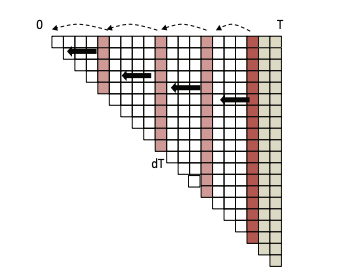
\includegraphics[height=5cm]{CRRpartitioned.png}
    \caption{A visualization of the parallelized CRR algorithm using partitioning. BLA BLA BLA lorem ipsum. MAKE YOUR OWN PICTURE OF THIS, OR CHECK IF THE FIGURES ARE OK TO USE UNDER COPYRIGHT}
    \label{fig:combined}
\end{figure}


\footnote{For what it's worth, the authors state that this can also be applied to American options by "filling in the intermediary nodes". I have been thinking about this for long now, and this still does not make sense to me. I am skeptical to claim that this is doable without having seen a better explanation on the matter. Hence, my performance analysis ignores the contribution of this step.}

Again, asymptotically, we still have $O(n^2)$ as we do computations for every node in the tree. The coefficient calculations is directly comparable to the actual option value calculations from the previous version, but we expect a factor $p$ speedup due to performing this work in parallel over all partitions. We then have to calculate the actual option values at all the nodes at the partition boundaries using \eqref{relative-prices}. The sum contains an amount of terms equal to the partition width plus one, $n/p+1$. Given enough parallel computing resources to calculate this sum for all the nodes simultaneously, this is in total an $O(n)$ operation. In practice, however, the dependency chain of the work has been reduced enough to reduce overall execution time, and the authors report a 2x speedup over a general parallel algorithm. Furthermore, they derive the optimal number of partitions $p$ for minimal execution time, and find it to be directly proportional to the square root of the amount of time steps, but inversely proportional to the square root of the latency of propagation between the partitions. Dividing the lattice into more partitions improves execution time due to parallelism up to a certain point, where the communication and boundary calculation overhead between the partitions exceed the former speedups. The paper compares this tradeoff by plotting execution time of an n=1000 size problem as a function of the number of partitions for different communication latencies (do I mention this, add it in the thesis or what?)\footnote{The original paper simplifies the analysis by only considering the communication overhead between partitions as opposed to also including the option value calculations at the boundaries. The conclusions, however, remain the same, as the choice of $p$ does not affect the computational cost of calculating the option values at the boundaries. More partitions means more boundaries to calculate in, but the smaller partition width means less summation terms. (Do I need some appendix deriving this stuff? This is my analysis based on the paper.)}.


\section{GPU Acceleration of Monte Carlo Methods} \label{sec:gpu-mc}
\subsection{Monte Carlo Methods}
Monte Carlo (MC) methods are a class of computational algorithms that approximate solutions to problems through random sampling. Unlike analytical and deterministic numerical methods that rely heavily on domain-specific mathematical theory, MC methods are relatively simple and model-agnostic. They depend primarily on the \emph{law of large numbers}, which states that the sample average tends toward the true expected value with increasing sample size \cite{Ross2020prob}. Therefore, with a well-chosen sampling distribution whose expectation matches the target quantity, the average of a large number of simulated outcomes provides a reliable approximation of the solution. While true random number generation is difficult, there exist many so-called pseudorandom number generation algorithms, whose deterministic sequences are statistically indistinguishable from true randomness. To achieve sampling from a specific probability distribution, the general approach is to first use a \emph{linear congruential generator} that samples numbers from a uniform distribution $U(0,1)$, and then apply a transformation to map these to the desired distribution. A common example is the Box-Muller transform for a standard normal mapping $U(0,1) \rightarrow N(0,1)$. \cite{gentle2003random}

Many software libraries contain easy-to-use random number generators from various distributions. This, coupled with the availability of affordable computing power, has made MC methods hugely popular for brute force problem solving across different domains. Their generality, however, still comes at a significant computational cost. While analytical and other numerical methods exploit problem-specific structure for a faster convergence, MC methods typically require a large number of iterations to produce accurate results. Consequently, MC methods are often employed for high-dimensional problems where traditional approaches fail or become exceedingly slow \cite{gentle2003random}. In derivatives pricing, MC methods are mostly used for exotic options with complex payoff structures, e.g. multi-asset options whose payoff depend on numerous underlying assets \cite{hull2016options,wilmott2013paul}.

Option pricing by MC simulation relies on the same risk-neutral valuation framework presented earlier in \cref{sec:risk-neutral-theory}. While the BSM model provides an analytical solution to a partial differential equation for the expected discounted payoff, the MC approach instead estimates this value numerically by computing the discounted average of many simulated option payoffs, each obtained from a risk-neutral stock price path \cite{boyle1977options}. The result is always an approximation, but converges toward the theoretical value as the number of simulated paths increases. The construction and dynamic maintenance of a replicating portfolio naturally extends to continuous-time models. The stock price dynamics used for MC simulations are often a discretized version of the \emph{geometric Brownian motion} process used in the continuous BSM model, which is also the behavior of the CRR model in the limit as $n \rightarrow \infty$. Under these assumptions, one can solve for the exact distribution of the stock price at a future time point $t$, and thus the discretization does not introduce an error. At each point in time, the stock price is updated according to
\begin{equation*}
S_{t+\Delta t} = S_t \cdot \exp \left( \nu \Delta t + \sigma \sqrt{\Delta t} \cdot \epsilon_i \right),
\label{eq:GBM-price}
\end{equation*}
where $\nu=r-\frac{1}{2}\sigma^2$ and $\epsilon_i \sim N(0,1)$. Hence, there is no need to use more than one time period unless the payoff function is path dependent, as for e.g. Asian options whose payoff is calculated using the average stock price over the holding period. In this case, much like the CRR algorithm, we get a better approximation with larger values of $n$ and smaller time steps. \cref{alg:MC-algo}, based on the implementation by Clelow and Strickland, demonstrates a generic MC implementation \cite{clelow1998implementing}. The algorithm has an asymptotic time complexity of $O(M \cdot n)$ as we run $M$ simulations, each $n$ periods long, and calculate the option payoff in each one. The payoff calculation complexity ranges from $O(1)$ for simpler options to $O(n)$ for more complex, path dependent options. 

\begin{algorithm}
\caption{MC Option Pricing}
\label{alg:MC-algo}
\textbf{Data:} $S_0$ (initial stock price), $K$ (strike price), $T$ (time to maturity), $r$ (risk-free rate), $n$ (time steps), $\sigma$ (volatility), $M$ (simulated paths), $\text{payoff}(\cdot)$ (payoff function)\\
\textbf{Result:} Option price at $t=0$\\

$\Delta t \gets T/n$\;
$\nu \gets r - 0.5 \cdot \sigma^2$\;
$\text{nudt} \gets \nu \cdot \Delta t$\;
$\text{sigsqrt} \gets \sigma \cdot \sqrt{\Delta t}$\;

Initialize $C_{\text{sum}} \gets 0$\;

/* Simulate $M$ stock price paths */\\
\For{$j \gets 1$ \KwTo $M$}{
    Initialize $S[0] \gets S_0$\;
    /* Simulate stock price path through $n$ time steps */\\
    \For{$i \gets 1$ \KwTo $n$}{
        Sample $\epsilon \sim \mathcal{N}(0,1)$\;
        $\ln S[i] \gets \ln S[i-1] + \text{nudt} + \text{sigsqrt} \cdot \epsilon$\;
        $S[i] \gets \exp(\ln S[i])$\;
    }
    /* Compute option payoff for the simulated path */\\
    $C_j \gets \text{payoff}(S[0..n])$\;
    $C_{\text{sum}} \gets C_{\text{sum}} + C_j$\;
}

/* Discount and average the payoffs */\\
$C_0 \gets \exp(-r \cdot T) \cdot \frac{C_{\text{sum}}}{M}$\;

\Return{$C_0$}\;
\end{algorithm}


\subsection{Naive GPU-acceleration}
MC simulation is considered an \emph{embarrassingly parallel} problem, since an accelerated version can be obtained by simply running the simulations in parallel without any further algorithm redesign. Instead, the difficulty shifts to maintaining the quality and independence of the random number streams generated in parallel. Because only a finite set of states can be represented in binary, a deterministic sequence (such as one produced by a pseudorandom number generator) must eventually repeat. Moreover, problems can arise even before this point if significant correlations exist between number streams. Therefore, a parallel MC implementation must partition the state space carefully to avoid these issues while still ensuring efficiency \cite{gentle2003random}. This necessitates the use of generators specifically designed for parallel architectures, where each thread can produce an independent and high-quality random stream without introducing statistical bias. Early GPU implementations, such as those by Howes and Thomas \cite{nguyen2007gpu}, had to manually construct such generators. Today, GPU libraries like cuRAND provide various parallel random number generators as standard functionality, eliminating the need for manual implementation.

Given the resources to run $m$ simulations in parallel, the time complexity could thus be reduced to $O(\frac{M}{m}\cdot n)$. The aforementioned authors \cite{nguyen2007gpu} compared the performance of both normal random number generation and MC pricing of exotic Asian and lookback options, using an Nvidia GeForce 8 GPU and AMD Quad Opteron 2.2 GHz CPU. A 26x speedup was achieved in pure random number generation, while a 59x and 23x speedup improvement were seen for MC pricing of Asian and lookback options respectively. These results show that even fairly naive GPU implementations of the early days (2007) achieved substantial speedups over multi-core CPU versions for MC option pricing, despite the inherent challenges of parallel random number generation. When examining the performance of the simulation computations in isolation (using constant values as opposed to random numbers), the theoretical speedups reached 118x for Asian options and 45x for lookback options. This indicates that RNG becomes a proportionally larger bottleneck on GPUs compared to CPUs. The choice of random number generator also depends on the option type and memory constraints, as some option payoffs require storing intermediate values in memory. In this example, the sum used for the average calculation in the Asian option can be accumulated in a single variable, leading to minimal memory requirements. This enabled the use of the faster Wallace RNG, which could not be used in the pricing of more memory-intensive lookback options that needed to store entire price paths.

\subsection{Further Hardware Optimization}
Unlike the CRR model, where algorithmic reformulation was necessary to expose hidden parallelism, Monte Carlo simulation presents a fundamentally different optimization challenge. The parallelism is already fully exposed at the algorithmic level -- each simulation path is completely independent, requiring no communication or synchronization with other paths. This embarrassingly parallel structure means that further speedups must come not from mathematical reformulation, but from efficiently mapping this abundant parallelism onto GPU hardware constraints. While techniques such as variance reduction methods and the use of quasi-random numbers can improve convergence rates \cite{clelow1998implementing}, they benefit any implementation equally and are thus not relevant to the scope of this thesis. Instead, further GPU acceleration requires addressing hardware-specific challenges, such as efficient random number generation, optimizing memory access patterns, and resource utilization. 

Liu et al.\ \cite{liu2010efficient} demonstrate several optimization strategies for further speeding up parallel MC option pricing. The problems they identified were mostly forms of inefficient memory access patterns and use of resources. The simplest optimization was to compress the working set -- that is, the amount of memory each thread must keep track of during simulation -- reducing reliance on slow global memory. The extent to which this is achievable heavily depends on the option type and choice of RNG \textbf{(if this sentence is MY thoughts, how do I separate it from citation?)}. Another common bottleneck is the memory bandwidth, for which reorganizing for coalesced accesses serves as a solution. The fixed amount of registers per streaming multiprocessor (SM) can also lead to sub-optimal parallelism if the implementation requires a high amount of registers in use per thread, leading to ``leaving parallelism on the table''. A proposed solution is to split the process into smaller GPU kernels, each responsible for sub-tasks (e.g. one for RNG, another for simulation). While this enables more efficient processor utilization, it comes at a cost of more global memory accesses between kernels. These techniques enabled a 43x speedup for exotic MC option pricing on an Nvidia Tesla C1060 GPU compared to an Intel 8-core Xeon 2.0 GHz CPU.

The authors also explore the practical case of large workloads where the threads compute multiple price paths, and the tradeoff between two such execution strategies. In ``path mode'' a thread computes its paths sequentially from start to finish. This minimizes memory usage and is well suited for homogeneous workloads like the paths for the same option. In contrast, ``slice mode'' divides the computations across time steps, and computes the corresponding simulation step for all paths. This is naturally more memory intensive as intermediary data is required for all the paths. On the other hand, slice mode handles heterogeneous workloads better, e.g. the case of distributing calculations for multiple options over the threads. If these options have different maturities, some path simulations will finish earlier than others, leading to control-flow \emph{warp divergence}\textbf{(mention this in GPU chapter first time, and no need to emph it here)}. Slice mode alleviates this by structuring the computations to minimize the cost of such divergence. \cref{fig:gpu-divergence} depicts the different execution modes and their effect on divergence. While these techniques were introduced in 2010 and GPU architectures have evolved significantly since then (e.g., with better warp scheduling and memory handling), the underlying tradeoffs between memory usage, synchronization, and parallel efficiency remain central to high-performance Monte Carlo implementations, even on modern GPUs. \cite{liu2010efficient}

\begin{figure}[htbp]
\centering
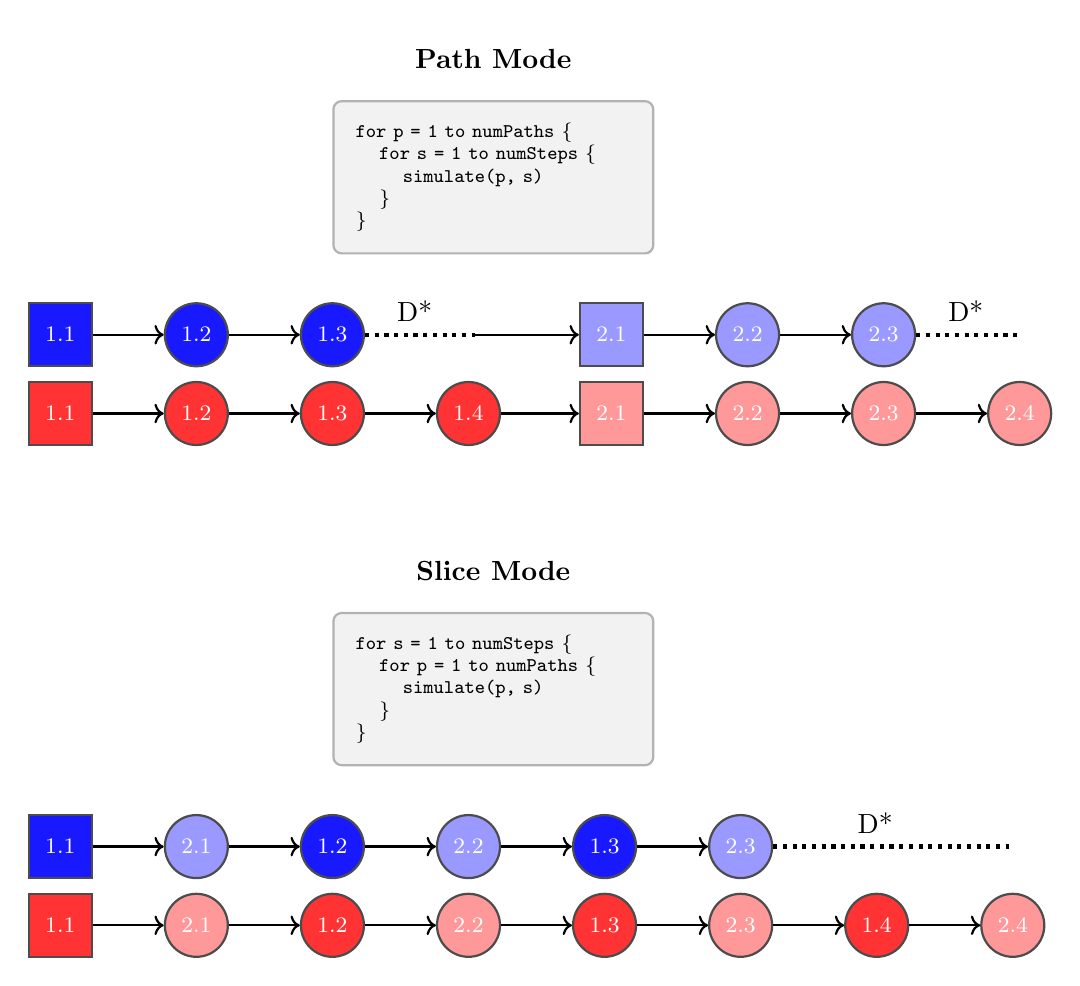
\begin{tikzpicture}[
    node distance=0.9cm,
    every node/.style={minimum size=0.8cm, font=\footnotesize, thick, draw=black!70, inner sep=0pt}
]

% Calculate center position
\def\centerx{6}

% Path Mode Title
\node[draw=none, font=\bfseries] at (\centerx, 9.5) {Path Mode};

% Path Mode Pseudocode
\node[draw=black!30, fill=gray!10, text width=3.5cm, align=left, font=\ttfamily\scriptsize, inner sep=8pt, rounded corners=3pt] at (\centerx, 8) {
for p = 1 to numPaths \{\\
\hspace{0.3cm}for s = 1 to numSteps \{\\
\hspace{0.6cm}simulate(p, s)\\
\hspace{0.3cm}\}\\
\}
};

% PATH MODE
% Thread 1 (Blue) - Path 1
\node[rectangle, fill=blue!90, text=white] (b11) at (0.5, 6) {1.1};
\node[circle, fill=blue!90, text=white, right=of b11] (b12) {1.2};
\node[circle, fill=blue!90, text=white, right=of b12] (b13) {1.3};

% Thread 2 (Red) - Path 1  
\node[rectangle, fill=red!80, text=white] (g11) at (0.5, 5) {1.1};
\node[circle, fill=red!80, text=white, right=of g11] (g12) {1.2};
\node[circle, fill=red!80, text=white, right=of g12] (g13) {1.3};
\node[circle, fill=red!80, text=white, right=of g13] (g14) {1.4};

% Dotted line and DIVERGENCE text after path 1
\draw[dotted, line width=1.5pt] (b13.east) -- ++(1.4,0) coordinate (b_dotted_end);
\node[draw=none, font=\normalsize] at (5, 6.3) {D*};

% Thread 1 (Blue) - Path 2 (lighter)
\node[rectangle, fill=blue!40, text=white] (b21) at (7.5, 6) {2.1};
\node[circle, fill=blue!40, text=white, right=of b21] (b22) {2.2};
\node[circle, fill=blue!40, text=white, right=of b22] (b23) {2.3};

% Thread 2 (Red) - Path 2 (lighter)
\node[rectangle, fill=red!40, text=white] (g21) at (7.5, 5) {2.1};
\node[circle, fill=red!40, text=white, right=of g21] (g22) {2.2};
\node[circle, fill=red!40, text=white, right=of g22] (g23) {2.3};
\node[circle, fill=red!40, text=white, right=of g23] (g24) {2.4};

% Dotted line and DIVERGENCE text after path 2
\draw[dotted, line width=1.5pt] (b23.east) -- ++(1.3,0);
\node[draw=none, font=\normalsize] at (12, 6.3) {D*};

% Arrows
\foreach \i/\j in {b11/b12, b12/b13, g11/g12, g12/g13, g13/g14,
                   b21/b22, b22/b23, g21/g22, g22/g23, g23/g24}
    \draw[->, thick] (\i) -- (\j);

% New arrows from path 1 to path 2
\draw[->, thick] (g14) -- (g21);
\draw[->, thick] (b_dotted_end) -- (b21);

% SLICE MODE
\node[draw=none, font=\bfseries] at (\centerx, 3) {Slice Mode};

% Slice Mode Pseudocode  
\node[draw=black!30, fill=gray!10, text width=3.5cm, align=left, font=\ttfamily\scriptsize, inner sep=8pt, rounded corners=3pt] at (\centerx, 1.5) {
for s = 1 to numSteps \{\\
\hspace{0.3cm}for p = 1 to numPaths \{\\
\hspace{0.6cm}simulate(p, s)\\
\hspace{0.3cm}\}\\
\}
};

% Thread 1 (Blue) - alternating colors
\node[rectangle, fill=blue!90, text=white] (sb11) at (0.5, -0.5) {1.1};
\node[circle, fill=blue!40, text=white, right=of sb11] (sb21) {2.1};
\node[circle, fill=blue!90, text=white, right=of sb21] (sb12) {1.2};
\node[circle, fill=blue!40, text=white, right=of sb12] (sb22) {2.2};
\node[circle, fill=blue!90, text=white, right=of sb22] (sb13) {1.3};
\node[circle, fill=blue!40, text=white, right=of sb13] (sb23) {2.3};

% Thread 2 (Red) - alternating colors
\node[rectangle, fill=red!80, text=white] (sg11) at (0.5, -1.5) {1.1};
\node[circle, fill=red!40, text=white, right=of sg11] (sg21) {2.1};
\node[circle, fill=red!80, text=white, right=of sg21] (sg12) {1.2};
\node[circle, fill=red!40, text=white, right=of sg12] (sg22) {2.2};
\node[circle, fill=red!80, text=white, right=of sg22] (sg13) {1.3};
\node[circle, fill=red!40, text=white, right=of sg13] (sg23) {2.3};
\node[circle, fill=red!80, text=white, right=of sg23] (sg14) {1.4};
\node[circle, fill=red!40, text=white, right=of sg14] (sg24) {2.4};

% Arrows
\foreach \i/\j in {sb11/sb21, sb21/sb12, sb12/sb22, sb22/sb13, sb13/sb23,
                   sg11/sg21, sg21/sg12, sg12/sg22, sg22/sg13, sg13/sg23,
                   sg23/sg14, sg14/sg24}
    \draw[->, thick] (\i) -- (\j);

% Single divergence - dotted horizontal line
\draw[dotted, line width=1.5pt] (sb23.east) -- ++(3,0);
\node[draw=none, font=\normalsize] at (10.85, -0.2) {D*};

\end{tikzpicture}
\caption{GPU warp divergence under heterogeneous workloads in path versus slice execution modes, as described by Liu et al. \cite{liu2010efficient}. Nodes represent simulation steps, and are labeled $(p,s)$ where $p$ is the path index and $s$ is the step index. $D*$ represents a section where warp divergence occurs. In path mode, threads simulate entire paths sequentially, causing divergence at each path boundary when the paths differ in numbers of steps. In slice mode, threads interleave simulation of the same step in all paths, resulting in only a single divergence point when shorter simulations complete. While both modes may theoretically incur the same total idle time, the higher number of control-flow divergence events in path mode introduces greater overhead, which can lead to worse performance under heterogeneous workloads. }

\label{fig:gpu-divergence}
\end{figure}

\section{Summary and Conclusions}  \label{sec:summary}
This thesis evaluates the potential and practical effectiveness of GPU acceleration for two widely used option pricing algorithms: The Cox-Ross-Rubinstein (CRR) model and Monte Carlo (MC) simulation. The aim was to give a holistic assessment of the inherent algorithms' amenability to parallelization, common implementation strategies, attainable speedup, and typical performance bottlenecks. The findings show that both models can benefit significantly from GPU acceleration, though the scale and optimization techniques depend heavily on the algorithm's structure. MC methods offer more straightforward and substantial performance improvements due to their inherently parallel structure, while CRR requires more restructuring efforts to fully leverage GPU capabilities. The results of the reviewed research are aggregated in \cref{tab:results-table}.

An algorithm's inherent dependency structure largely determines both its parallelization potential and the strategies required for such optimizations. The CRR model, which operates through backward induction on a recombining lattice, is inherently sequential across time steps. This limits parallelization to computations within each time step. MC methods, by contrast, simulate independent price paths, making them ideally suited for parallelization. This is supported by the data: the naive CRR-GPU implementation achieved an approximately 10x speedup over a single-core CPU \cite{pharr2005gpu}, while the MC-GPU version achieved 23-59x speedups despite being benchmarked against a more modern quad-core CPU \cite{nguyen2007gpu}. Regardless of the method chosen, these straightforward GPU versions yield substantial gains relative to implementation effort, making them a clear improvement over sequential CPU versions. Scalability is eventually limited by bottlenecks -- thread communication latency for CRR and memory constraints for MC, particularly in RNG selection for memory-intensive option types.

Given these distinct characteristics, the algorithms present different optimization opportunities. For CRR, the dependency chains motivate algorithmic reformulation to expose additional parallelism. MC methods already expose parallelism to a high degree, hence optimization efforts are more focused on better utilization of the hardware. Ganesan et al. \cite{ganesan2009acceleration} exemplify the algorithmic reformulation approach for CRR by partitioning the time axis and computing relationship coefficients in parallel, effectively working around the sequential dependencies. They achieved a 2x speedup over a naive GPU version. For MC methods, Liu et al. \cite{liu2010efficient} implement hardware-conscious optimizations, including memory coalescing and minimizing warp divergence, for a 43x total speedup over a sequential version. These examples illustrate the key principle that the algorithm's inherent structure determines which optimization strategies are available. However, practical considerations of implementation difficulty and expected gains ultimately decide which path to pursue.

While the results indicate that MC methods tend to benefit more from GPU acceleration, they should not dictate algorithm choice. In practice, algorithm selection depends on multiple factors: option type, available hardware, and other individual requirements and constraints. For example, vanilla options are rarely priced using MC methods, as these are generally outperformed by analytical or lattice-based models. A general approach would thus be to first select an appropriate model that fits the requirements, and then to attempt GPU acceleration. As per the results, significant speedups can be achieved even with simpler implementations, and thus leveraging GPU capabilities should always be considered (along with other potential optimization strategies) in algorithmic option pricing. This becomes especially relevant for high-throughput tasks, such as bulk pricing or risk calculations across large portfolios.

An important caveat is that the analyzed research spans 2005-2010. Much of the cutting-edge research often remains proprietary within financial institutions that guard their competitive advantages, making it difficult to review the most recent developments in the field. GPU architectures have also evolved dramatically since then, largely driven by the massive demand for AI computing. Modern GPUs feature improved memory hierarchies, better divergence handling, and enhanced support for general-purpose computing, mitigating several of the mentioned bottlenecks and perhaps revealing new ones. Similarly, modern multi-core CPUs certainly enable faster baseline solutions than those in the original studies. While details change, the fundamental principle remains -- maximal GPU utilization is achieved both through algorithmic design and optimizing on the hardware level. Future work could examine these algorithms on modern architectures, and perform more direct comparisons. Expansive research could also be done on GPU acceleration of other models, such as finite difference or machine learning-based methods.


\begin{table}[h]
\centering
\begin{threeparttable}
\caption{Empirically measured GPU speedups for selected option pricing models. Reported results are based on real implementations and vary in terms of baseline architecture and research methodology. While not directly comparable, they provide indicative insight into practical performance improvements when interpreted with appropriate caution.}


\label{tab:results-table}
\begin{tabular}{lrp{4.5cm}p{4.5cm}}
\toprule
\textbf{Algorithm} & \textbf{\shortstack{Reported\\Speedup}} & \textbf{Strategy} & \textbf{Bottleneck} \\
\midrule
CRR\\
\cmidrule{1-2}
Naive & 10x\tnote{1} & Parallelization within time steps & Synchronization latency between time steps \\
Partitioned & 2x\tnote{2} & Additional parallelization across time periods & Inter-partition communication \\
\addlinespace 
MC\\
\cmidrule{1-2}
Naive & 23–59x\tnote{3} & Parallel simulation paths & random number generation, memory bandwidth \\
Optimized & 43x\tnote{4} & Memory coalescing, register reuse, warp divergence minimization & Memory bandwidth and register pressure \\
\bottomrule
\end{tabular}
\begin{tablenotes}
\footnotesize
\item[1] NVIDIA GeForce 6800 Ultra vs single-core 2.0GHz CPU (2005). \cite{pharr2005gpu}
\item[2] NVIDIA Tesla C1060 vs CRR Naive on the same architecture (2009) \cite{ganesan2009acceleration}.
\item[3] NVIDIA GeForce 8800 vs 4-core 2.2GHz CPU (2007). \cite{nguyen2007gpu}
\item[4] NVIDIA Tesla C1060 vs 8-core 2.0GHz CPU (2010). \cite{liu2010efficient}
\end{tablenotes}
\end{threeparttable}
\end{table}

\cleardoublepage

% Start of Appendices
\appendix
\section{Derivation of Risk-Neutral Probability Form}  % For 
\label{appendix:risk_neutral_derivation}

In this appendix, we derive the risk-neutral probability form of the one-period binomial model option pricing formula.

\begin{align}
&\text{Starting from \eqref{eq:replicating-portfolio}:} \nonumber\\[0.7em]
&\frac{f_u - f_d}{S_0(u-d)}S_0 + \frac{f_d \cdot u-f_u \cdot d}{(u-d)(1+r)} \nonumber\\[0.7em]
&=\frac{f_u - f_d}{u-d} + \frac{f_d \cdot u-f_u \cdot d}{(u-d)(1+r)} \nonumber\\[0.7em]
&=\frac{(f_u - f_d)(1+r)}{(u-d)(1+r)} + \frac{f_d \cdot u - f_u \cdot d}{(u-d)(1+r)} \nonumber\\[0.7em]
&=\frac{f_u(1+r) - f_d(1+r) + f_d \cdot u - f_u \cdot d}{(u-d)(1+r)} \nonumber\\[0.7em]
&= \frac{f_u[(1+r) - d] + f_d[u - (1+r)]}{(u-d)(1+r)} \nonumber\\[0.7em]
&= \frac{1}{1+r} \cdot \frac{f_u[(1+r) - d] + f_d[u - (1+r)]}{u-d} \nonumber\\[0.7em]
&= \frac{1}{1+r} \left( f_u \cdot \frac{(1+r) - d}{u-d} + f_d \cdot \frac{u - (1+r)}{u-d} \right)\nonumber
\end{align}

This final form reveals the risk-neutral probabilities: $\tilde p = \frac{(1+r) - d}{u-d}$ and $\tilde q = 1-\tilde p = \frac{u - (1+r)}{u-d}$.

The no-arbitrage condition ensures $\tilde p$ and $\tilde q$ are correctly bounded by 0 and 1. If $1+r > u$, investors could profit by shorting the stock and investing in the risk-free asset. Conversely, if $d > 1+r$, they could earn guaranteed profits. Therefore, $d \leq 1+r \leq u$ must hold, which leads to $0\leq \tilde p, \tilde q \leq 1$. Furthermore, $\tilde p + \tilde q = 1$. Thus, our risk-neutral probabilities form a valid probability distribution over the two possible outcomes.





\phantomsection

\addcontentsline{toc}{chapter}{\bibname}
\bibliographystyle{IEEEtran}
\bibliography{bibliography.bib}


\end{document}